\documentclass[11pt]{article}

\usepackage[portuguese]{babel}
\usepackage[T1]{fontenc}
\usepackage[utf8]{inputenc}
\usepackage{amsmath}
\usepackage{graphicx}
\usepackage{subfig}
\usepackage[colorinlistoftodos]{todonotes}
\usepackage{listings}
\usepackage{color} 
\usepackage{float}
\usepackage[font={footnotesize}]{caption}
\usepackage{xcolor,colortbl}
\usepackage{array}
\usepackage{fixltx2e}
\setcounter{secnumdepth}{4}

\linespread{1.3}
\usepackage{indentfirst}
\usepackage[top=2cm, bottom=2cm, right=2.5cm, left=2.5cm]{geometry}



\begin{document}


\begin{titlepage}
	\begin{center}
		
		\hfill \break
		\hfill \break
		
		
\includegraphics[width=0.3\textwidth]{./logo}~\\[1cm]
		
		\textsc{\Large Mestrado Integrado em Engenharia Electrotécnica e de Computadores}\\[1.5cm]
		\textsc{\huge Sistemas Electrónicos de Processamento de Sinal}\\[0.25cm]
		
		{\huge \bfseries BPSK Modem \\[1.2cm]}
		
		Grupo n.º 2/3 \vspace{0.3cm}
		
		\begin{tabular}{l r}
			André Filipe Barroso Cerqueira \hspace{1mm} & n.º 65144 \\
			Guilherme Branco Teixeira \hspace{1mm} & n.º 70214  \\
			João André Catarino Pereira & n.º 73527
		\end{tabular}
		
		\hfill
		\hfill
		
		segunda-feira 15h30 - 18h30, LE1
		
	
		\vfill
		
		{\large Lisboa, 17 de Abril de 2015} 
		
	\end{center}
\end{titlepage}
\pagenumbering{gobble}
\clearpage

	\footnote{As linhas de código apresentadas durante o relatório têm como objectivo demonstrar a maneira de raciocinar na resolução de problemas, não representando uma cópia exata do código usado em laboratório, podendo até, serem consideradas \textit{pseudo-código}}
	
\tableofcontents
\pagebreak

\clearpage
\pagenumbering{arabic}

\section{Introdução}

Este trabalho consiste na primeira parte do projecto de laboratório da cadeira: desenvolvimento de um modem de $Binary$ $Phase$ $Shift$ $Keying$ (BPSK). 

Teve como objectivo a familiarização com o ambiente de desenvolvimento integrado de DSP que consiste nas placas de desenvolvimento DSK TMS320C6416 e DSK TMS320C6713 da $Texas$ $Instruments$ e no software de desenvolvimento $Code Composer Studio v5.5$. Para tal correram-se dois projectos exemplo (sine8\_buf e loop\_intr) e, usando as ferramentas de debug, alteraram-se certos parâmetros de forma a observar os efeitos nos sinais resultantes. Também se consolidaram os conhecimentos adquiridos desenvolvendo dois mini projectos: um oscilador sinusoidal controlado numericamente e o modulador do modem BPSK.

%objectivo do laboratorio
%
%o que foi feito
%
%o q o relatorio vai falar

\section{Projecto}

\subsection{Projectos de Demonstração}
Foram analisados dois projetos de demonstração com o intuito de familiarizar com os equipamentos e as principais rotinas do projeto.

\subsubsection{sine8\_buf}
\label{sec:sine8}
O objectivo deste projeto é representar a função sinusoidal, multiplicada por um determinado ganho, através de um conjunto de amostras que equivalem a um período da mesma, repetindo nos períodos seguintes esse mesmo conjunto. Este procedimento é realizado através da rotina de interrupção presente no programa. 

Ao analisar o código deste projeto à primeira vista podemos concluir logo que este usa uma frequência de amostragem de 8 kHz , tem um ganho $G=10$ predefinido e usa 8 amostras para representar a sinusoide. Depois de observar a sinusoide no osciloscópio variou-se o ganho a fim de perceber a sua influência e também o seu limite.
 
Para compreender o limite desta sinusoide é necessário ter em conta que se usa o formato de vírgula fixa Q15 para as amostras da sinusoide. Este formato tem como limite o valor $(2^{15}-1) = 32767$. Considerando o valor máximo da sinusoide, se multiplicarmos a mesma por um ganho G=33 obtemos um valor superior ao permitido pelo formato Q15, fazendo com que nesses pontos o valor da sinusoide "caia".     

\subsubsection{loop\_intr}\todo{ALTERAR}
\label{sec:loop}
Este projeto tem como objectivo fornecer-nos um template para os próximos projetos, em termos de comunicação com a placa e rotina de interrupção. Pode-se observar nas últimas linhas de código como se liga os sinais de entrada e saída aos canais da placa.

%interpretar!!
No projeto anterior observou-se os efeitos de overflow de uma variável. Neste observam-se os efeitos de aliasing (ou não, não me recordo se o DSP tem um filtro anti-aliasing à entrada)  devido ao sinal de line-in ter a mesma frequência que a frequência de amostragem. Se havia anti-aliasing, a partir dos 4khz deixariamos de ver uma sinusoide com os 3.3V. Não fizemos a experiência de mudar para sinal quadrado e variar a frequência, mas provavelmente nao iamos ver um sinal quadrado pois o espectro (infinito) deste teria que ser filtrado pelo anti-aliasing filter.

\subsection{BPSK}
Este projeto é constituído por duas partes, a primeira é um oscilador controlado numericamente e a segunda é um transmissor BPSK. Devido à existência de um inversor na placa utilizada deu-se, ao longo deste projeto, atenção ao efeito do inversor nos sinais, como se poderá observar nas próximas secções.

\subsubsection{P1. Oscilador controlado numericamente}

Usa-se o projeto descrito na secção \ref{sec:loop} como base para a construção de um oscilador controlado numericamente (\textit{NCO}). Um \textit{NCO} é um gerador de sinal digital que cria uma forma de onda discretamente representada no tempo e na amplitude. O \textit{NCO} terá as seguintes características:

\begin{table}[H]
	\centering
	\caption{Características do \textit{NCO} a construir.}
	\label{tab:NCO-car}
\begin{tabular}[c]{|l||c|c|}
	\hline \textbf{Parâmetro} & \textbf{Símbolo} & \textbf{Valor} \\ 
	\hline Frequência de amostragem & $ f_{s} $ & $ 16 kHz $ \\ 
	\hline Frequência mínima & $ f_{min} $ & $ 2 kHz $ \\ 
	\hline Frequência máxima & $ f_{max} $ & $ 6 kHz $ \\ 
	\hline
\end{tabular}
\end{table}

O projeto de construir o \textit{NCO} seguiu os seguintes passos que estão posteriormente desmitigados:

\begin{enumerate}
	\item Oscilador de Relaxamento (Integrador de Rampa). %Secção \ref{para:P1-1}.
	\item Look-up-table (LUT). %Secção \ref{para:P1-2}.
	\item Obtenção do sinal sinusoidal através da LUT.% Secção \ref{para:P1-3}.
	\item Criação de duas variáveis para controlar a frequência e amplitude do sinal sinusoidal. %Secção \ref{para:P1-4}.
	\item Utilização do sinal de entrada para controlar a frequência do sinal. %Secção \ref{para:P1-5}.
	\item Teste do oscilador com uma onda quadrada à entrada para observar o sinal modulado.  %Secção \ref{para:P1-6}.
	\item Melhoria da qualidade do oscilador com interpolação linear. % Secção \ref{para:P1-7}.
	\item Comparação dos espectros com e sem interpolação.%  Secção \ref{para:P1-8}.
\end{enumerate}
\pagebreak

\textbf{P1-1}

 Visto que a placa usada no laboratório (DSK TMS320C6713) tem $1 V$ de amplitude máxima na saída, foi usado o formato Q15 para representar o sinal de saída, pois um sinal representado em Q15 tem amplitude máxima de $2^{15}-1 = 32767 $.

Para construir um Oscilador de Relaxamento foi criado um programa que aumenta por a cada ciclo o sinal à saída de modo a que este tenha o comportamento de uma rampa. Este incremento tem de tomar um valor, que por agora se vai considerar constante, tal que $32767$ seja seu múltiplo. Ao verificar a tabela \ref{tab:NCO-car}, podemos chegar aos seguintes valores de incremento com as suas frequências correspondentes:


\begin{table}[H]
	\centering
	\caption{Valores a atribuir ao incremento do sinal na saída.}
	\label{tab:incrementos}
	\begin{tabular}[c]{|l||c|}
		\hline \textbf{Frequência de saída($f_0$)} & \textbf{Incremento($\Delta$)}\\ 
		\hline $ 2 kHz \quad (f_{min}) $ & $ 8192 $\\ 
		\hline $ 4 kHz $ & $ 16384 $  \\ 
		\hline $ 6 kHz \quad (f_{max}) $ & $ 24576 $ \\ 
		\hline
	\end{tabular}
\end{table}

Os valores calculados na tabela \ref{tab:incrementos} foram calculados através da seguinte fórmula:

\begin{equation}
 f_{0}= \frac{\Delta}{2A}f_{s} \Leftrightarrow \Delta= 2A\frac{f_{0}}{f_{s}} \hspace{3 mm}, A=32767
\end{equation}

Foi então possível obter as seguintes rampas com diferentes frequências:


\begin{figure}[H]
	\centering
	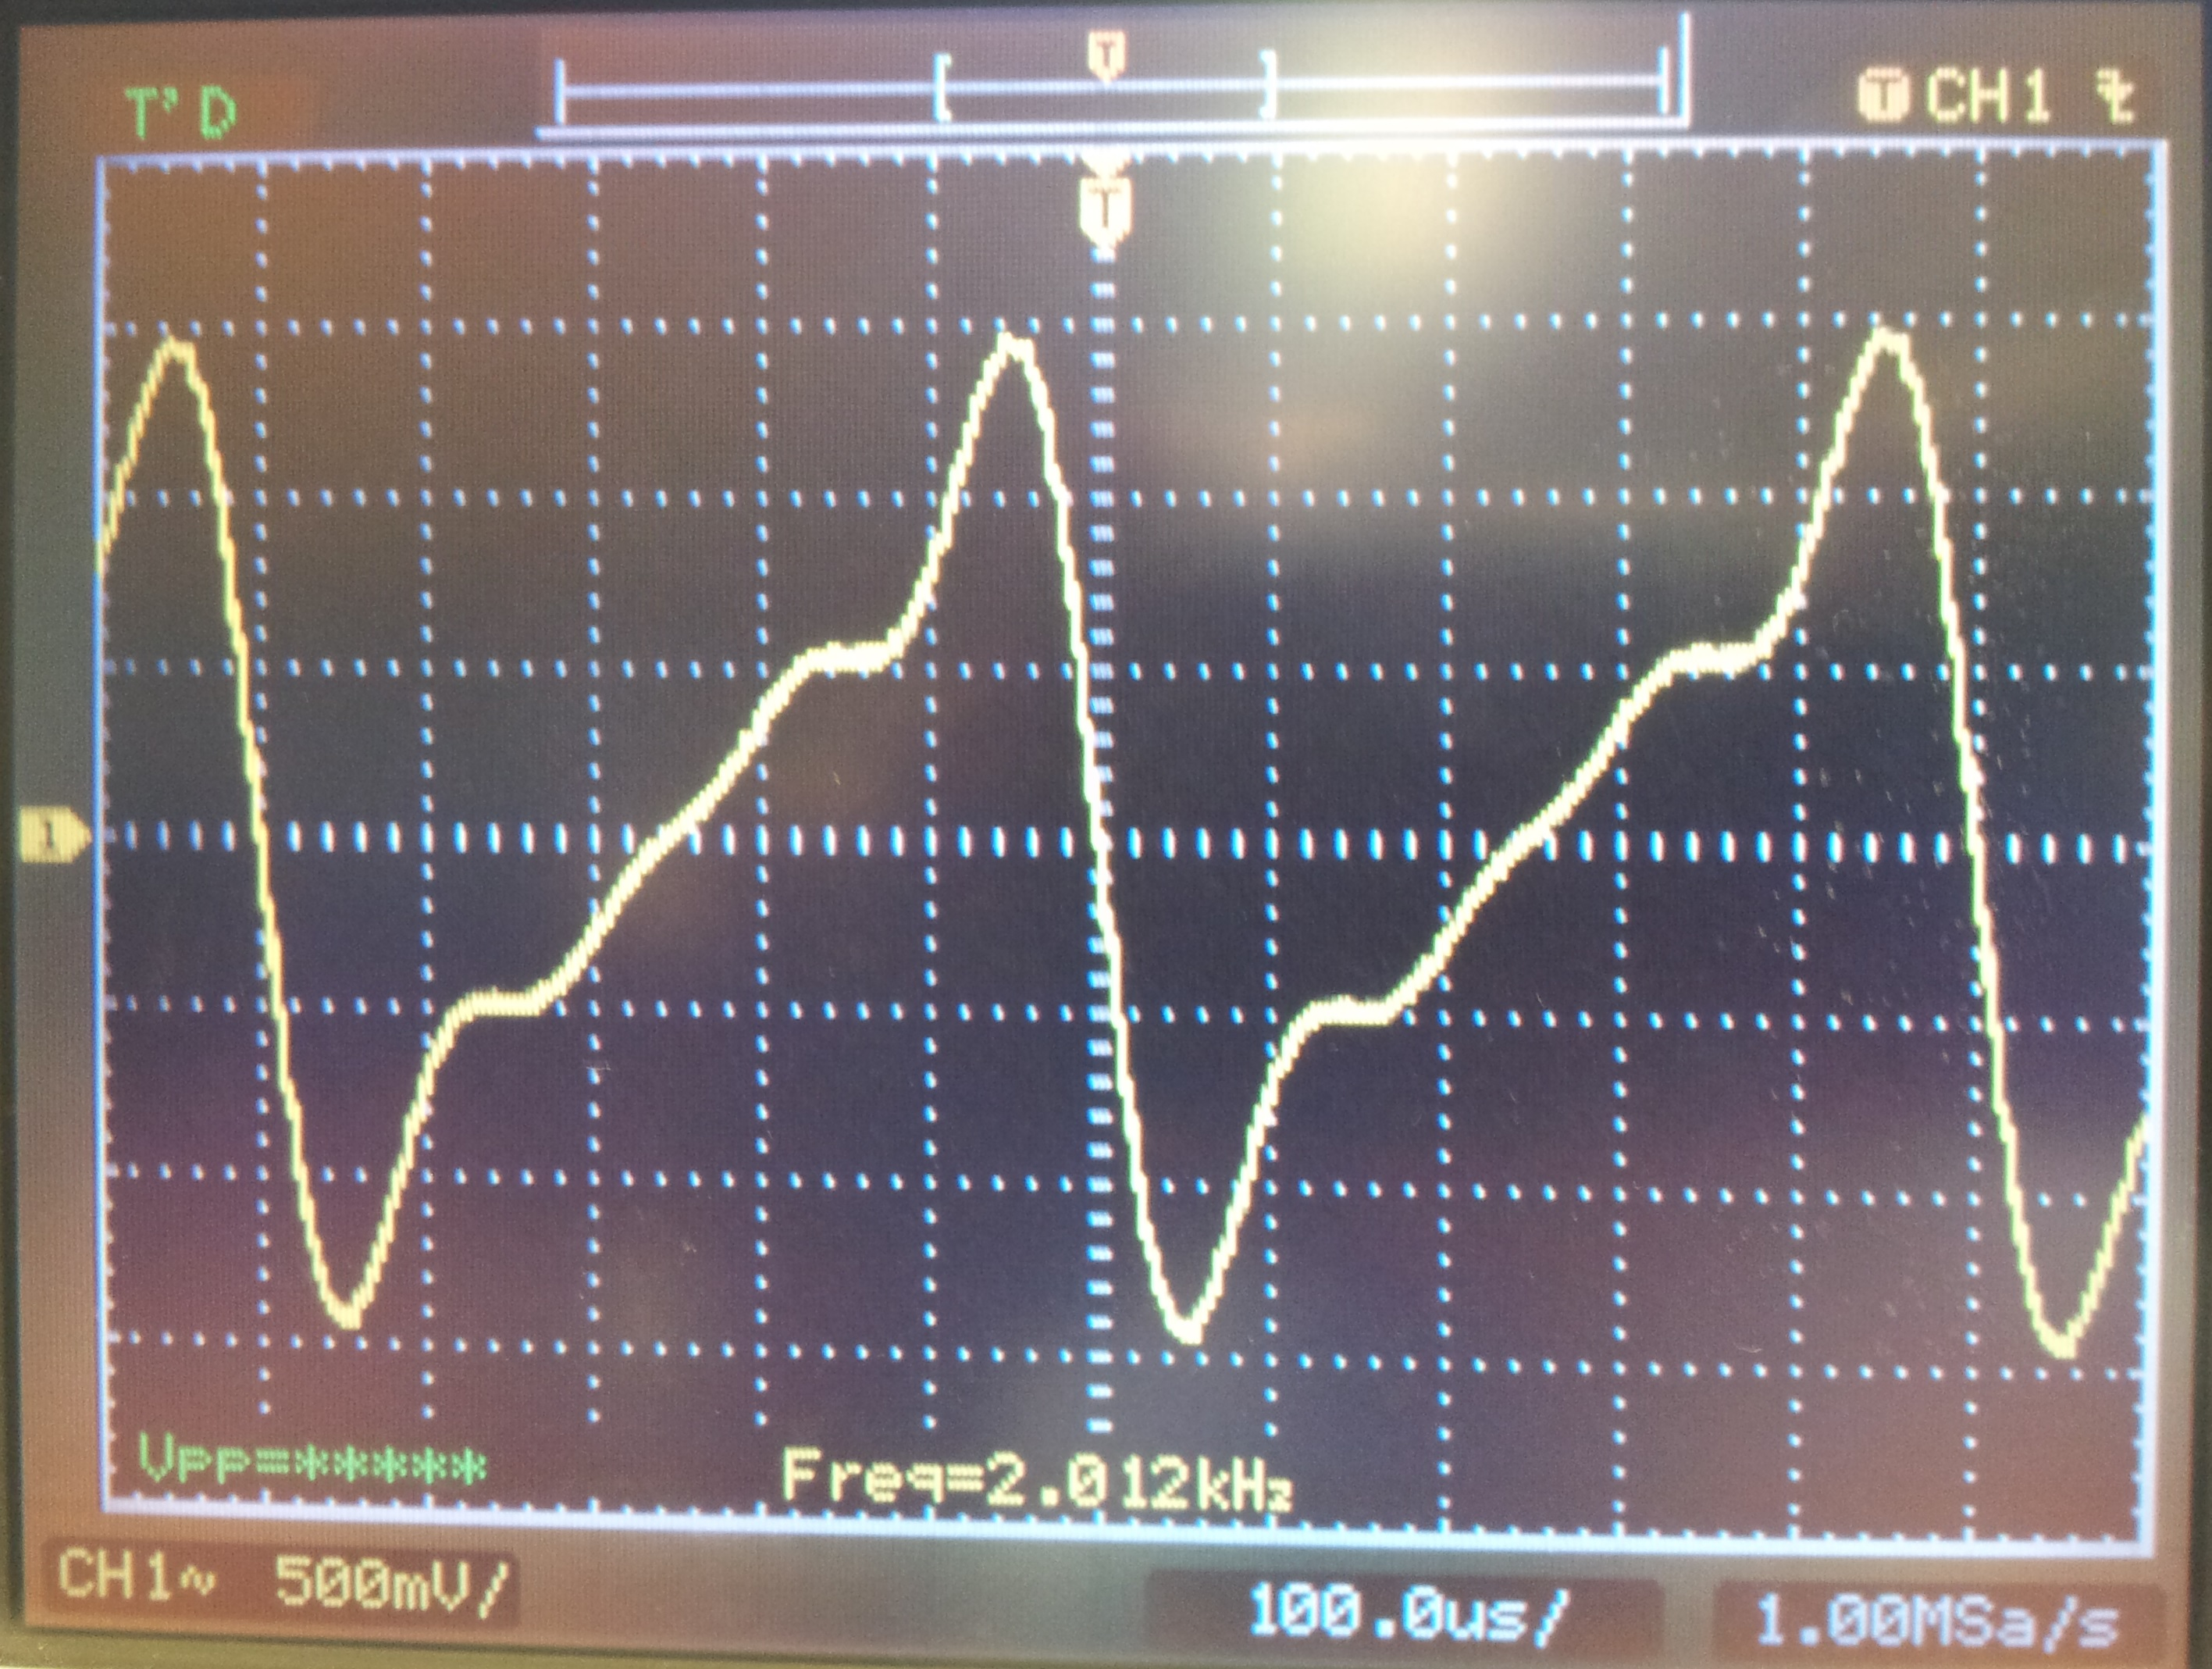
\includegraphics[width=0.5\textwidth]{./P1_2kHz}~\\
	\caption{Rampa com frequência de $ 2 kHz $}
\end{figure}


\begin{figure}[H]
	\centering
	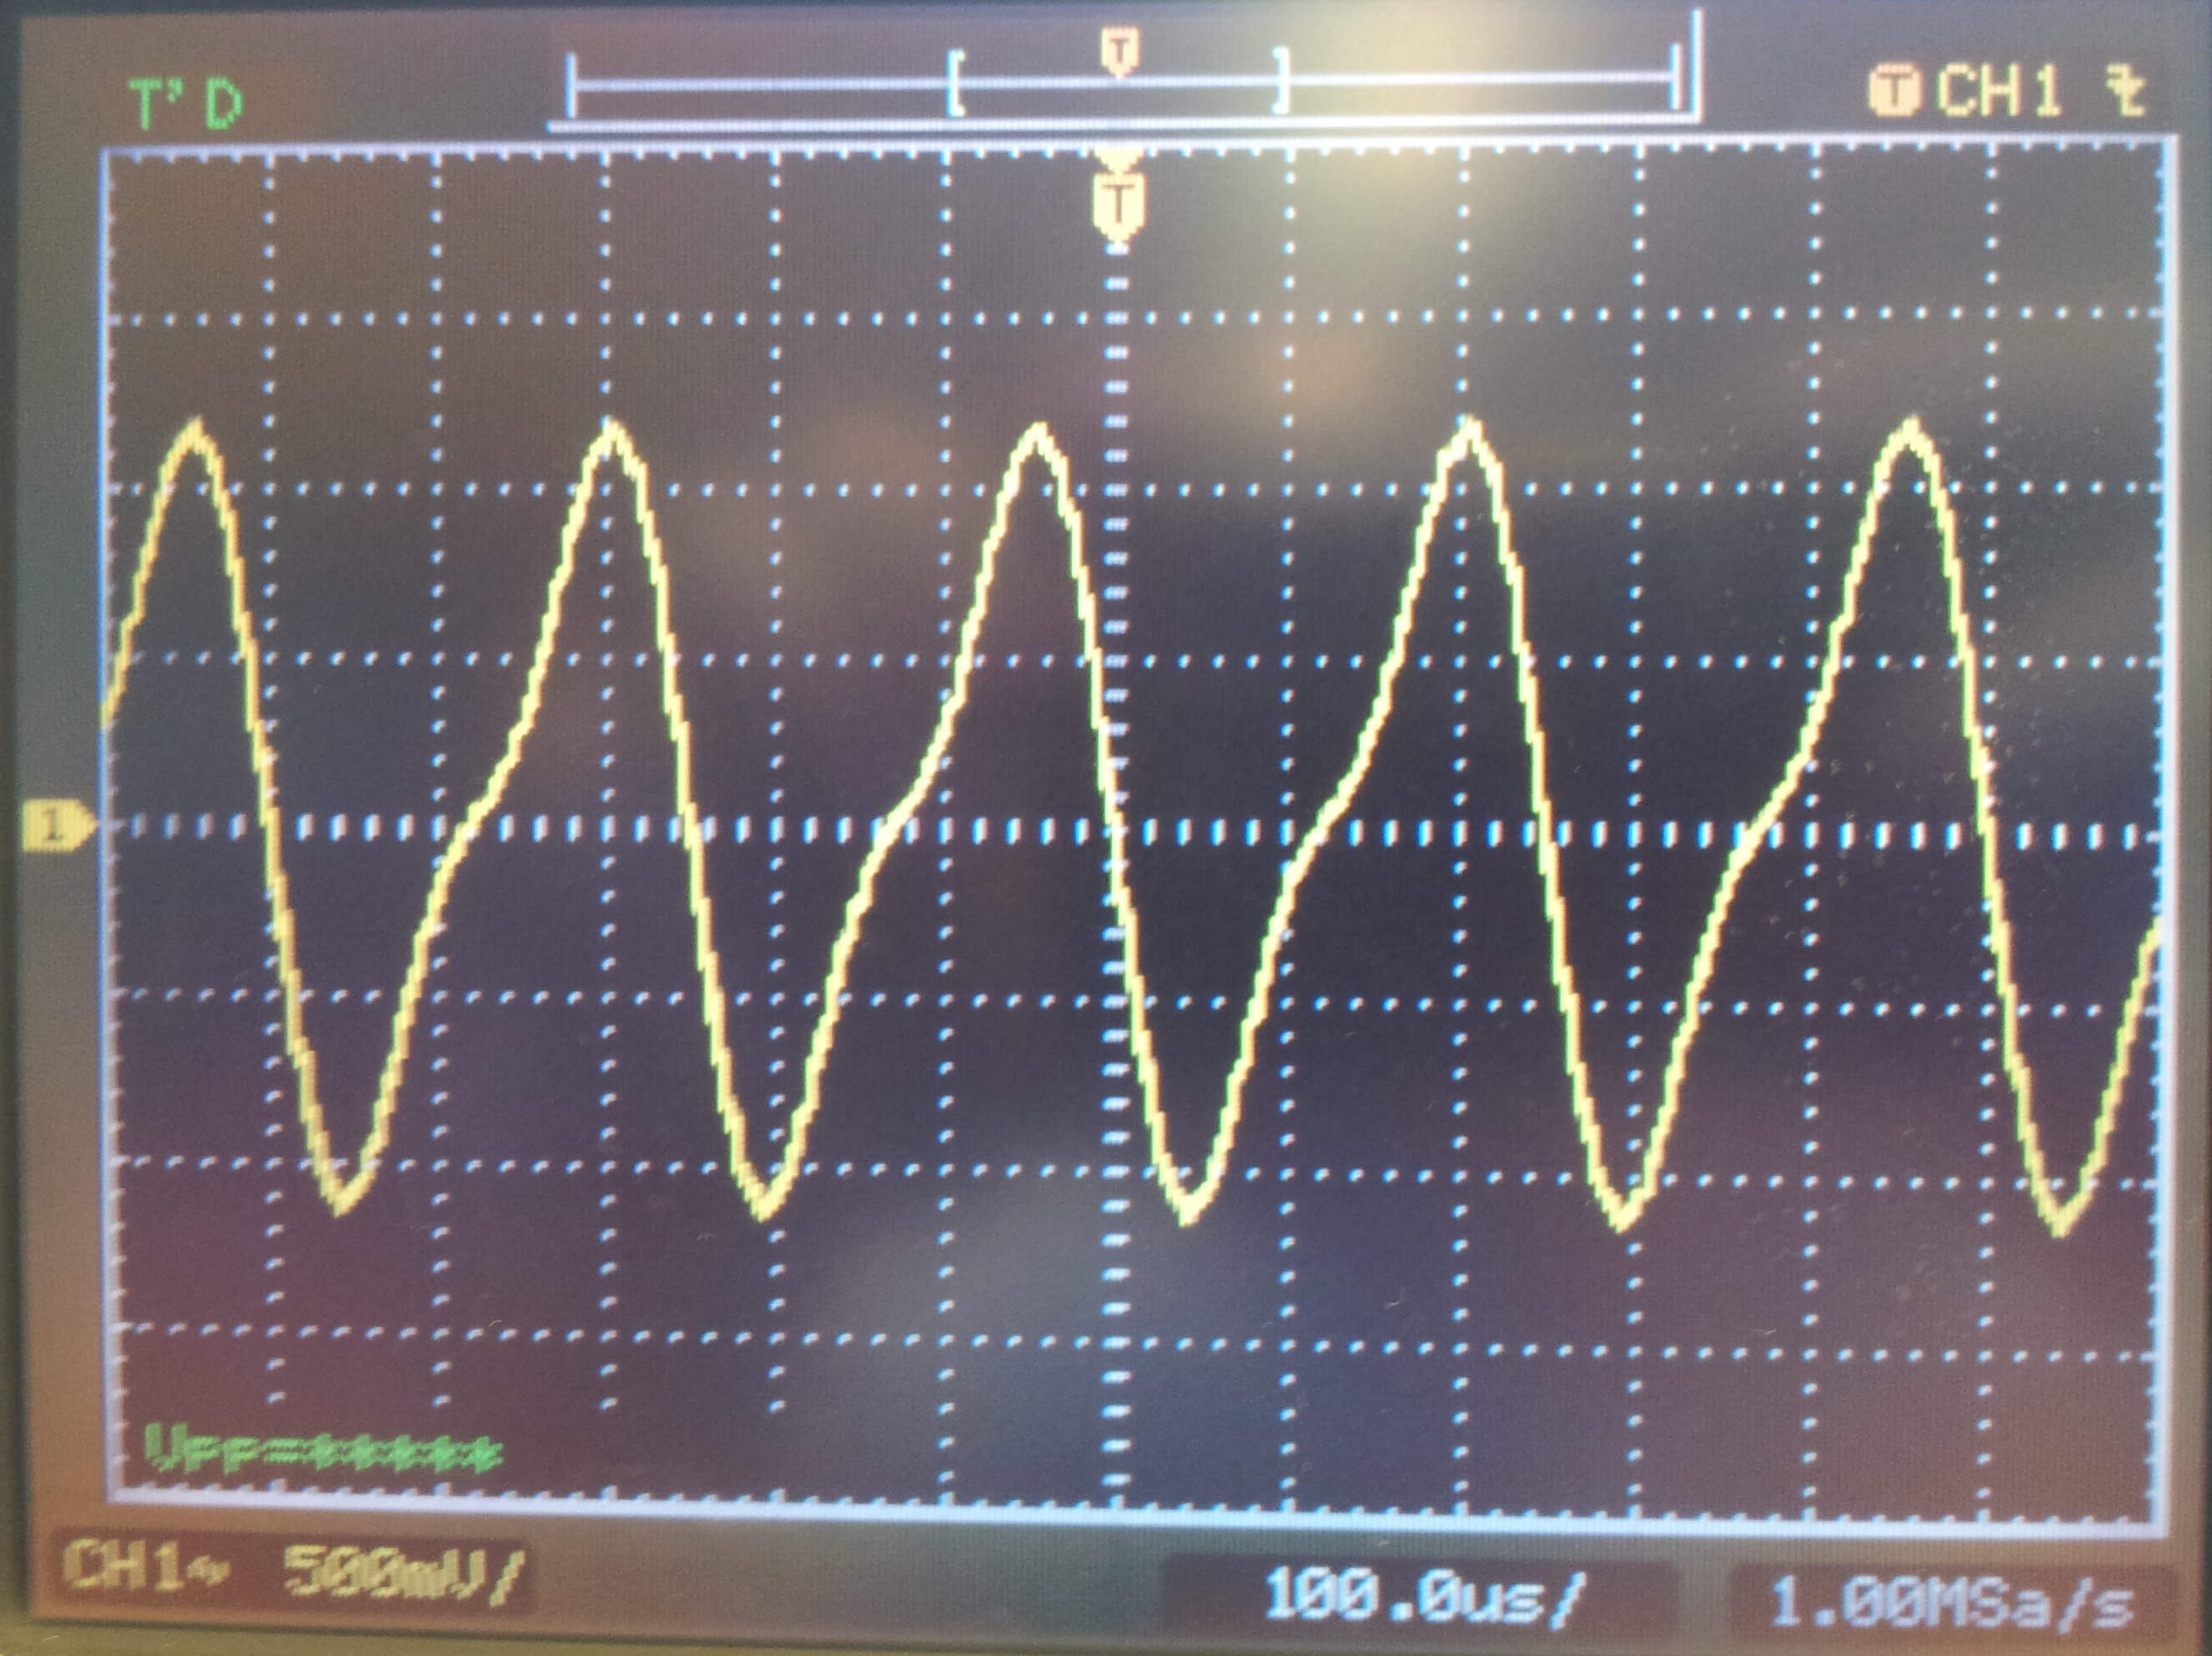
\includegraphics[width=0.5\textwidth]{./P1_4kHz}~\\
	\caption{Rampa com frequência de $ 4 kHz $}
\end{figure}
Ao observar as duas rampas pode-se constatar que para uma frequência mais baixa, ou seja, um incremento menor, a rampa apresenta mais "degraus" e um menor declive. Um incremento menor na rampa significa um maior número de amostras da mesma dentro do intervalo possível, o que reduz o declive da rampa. É de salientar que devido à presença do inversor da placa foi introduzido o simétrico da rampa no canal de modo a observar esta no sentido correto.
\vspace{2 mm}

\textbf{P1-2}

Foi criada uma tabela (LUT) com os valores em Q15 de meio ciclo de um seno de modo a que seja possível ir retirar os seus valores para criar um sinal sinusoidal. Esta tabela tem 32 valores e foi construída com a seguinte equação:

\begin{equation}
32767*\sin \dfrac{n \pi}{32},  \quad \quad n=0,1,2,...,31
\end{equation}
Para calcular apenas meio ciclo do seno, é necessário ter 32 valores pertencentes ao intervalo $[0,\pi]$ na fase. Assim, é necessário restringir a fase a esse intervalo através da divisão observada na expressão, $\frac{n \pi}{32}$. O produto do seno pelo valor 32767 é a conversão do seno para Q15. 

Não se multiplica por $2 ^{15}=32768$ pois os sinais estão em complemento para dois, o que significa que para o máximo do seno, esta LUT ultrapassaria o limite do formato, o que causaria o corte dessa amostra no sinal.
\vspace{2 mm}

\textbf{P1-3}

Usando como base a rampa criada na secção P1-1 para indexação da LUT criada na secção P1-2, foi possível criar um sinal de uma sinusoide.

De acordo com o projeto, a rampa é representada num formato Q10, com 1 bit sinal, 5 bits inteiros e 10 bits fraccionários. 
Para a indexação são usados os 5 bits inteiros, ou seja, os 5 mais significativos (excluindo o bit de sinal) do sinal da rampa, esses 5 bits irão indexar e escolher qual o valor da tabela de LUT a usar para criar a sinusoide. 

Este processo foi efetuado com o seguinte pedaço de código dentro do ciclo:

\begin{lstlisting}
	rampa=rampa+delta;    //Criar a rampa
	index=rampa>>10;
	index=31 & index;         //Usar apenas 5 bits
	sinusoide=LUT[index];
\end{lstlisting}

Como se pode observar, para isolar os 5 bits inteiros fez-se dez \textit{shifts} direitos de maneira a ter um sinal apenas com zeros, o bit sinal e esses 5 bits encostados à direita. A seguir aplicou-se uma máscara constituída por uma AND com 31, de maneira a retirar o bit sinal e finalmente isolar num sinal o índice pretendido da LUT. Com o índice é uma questão de aceder à tabela e obter \textit{y1}, neste caso representado pelo sinal \textit{sinusoide} (Figura \ref{fig:sen2k}).

\begin{figure}[H]
	\centering
	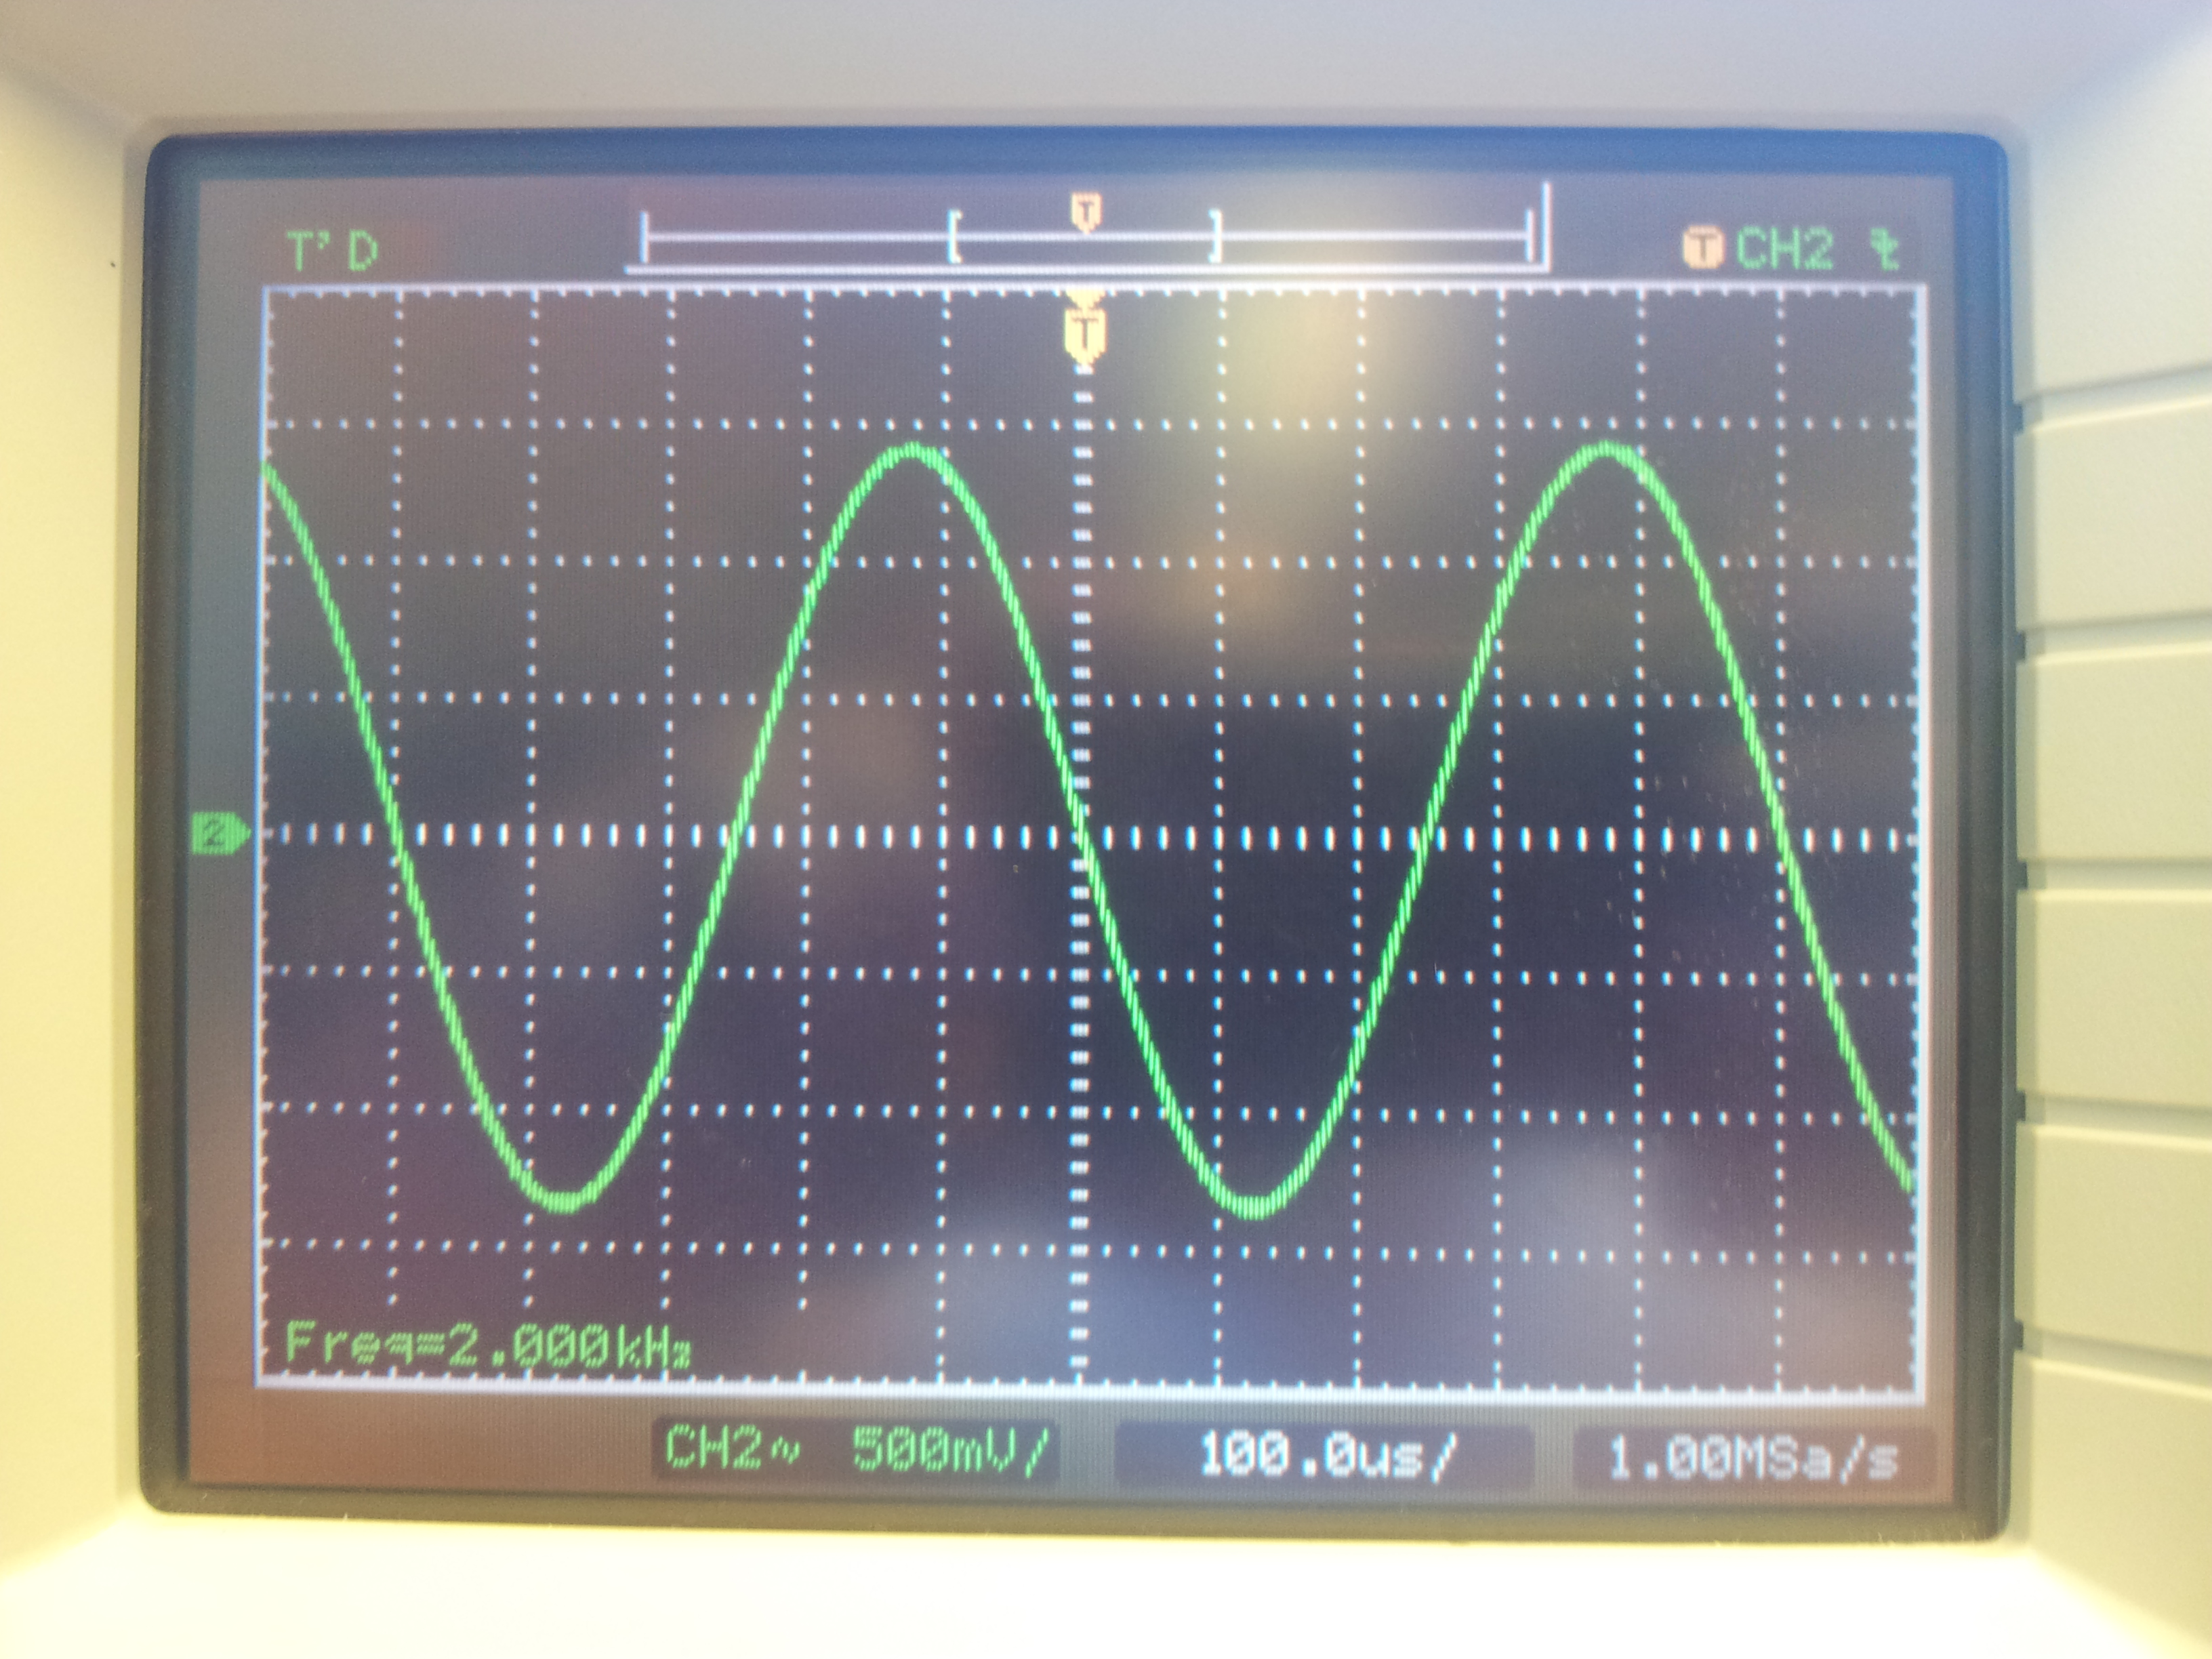
\includegraphics[width=0.5\textwidth]{./P1_1seno}~\\
	\caption{Sinal sinusoidal criado de $ 2 kHz $.}
	\label{fig:sen2k}
\end{figure}

Como se pode observar na figura foi possível criar um sinal aproximadamente sinusoidal através de uma LUT indexada por uma rampa. Nesta figura não é possível notar mas quando se aproxima mais o sinal no osciloscópio verifica-se pequenos degraus ao longo do sinal, que simbolizam a aproximação obtida através das amostras.
\vspace{2 mm}

\textbf{P1-4}

%variaveis vs sinais
Foram criadas duas variáveis para fosse possível controlar a frequência e a amplitude do sinal à saída, \textit{delta} e \textit{ampl}, respectivamente.

A primeira variável foi já antes referida, nas secções P1-1 e P1-3. Esta variável, caso alterada irá alterar a frequência da rampa, e por consequência, a frequência do sinal de saída. Como se pode observar na tabela \ref{tab:incrementos}, esta variável terá como limite máximo o valor $ 24576 $ e como limite mínimo $ 8192 $ devido às frequências mínima e máxima. Podemos também concluir que quanto maior for esta variável, maior a frequência do sinal de saída, tal como se o seu valor diminuir, a frequência de saída irá diminuir também.

A segunda variável (\textit{ampl}) foi criada com o propósito de modelar a amplitude do sinal de saída. Esta causou mudanças mais significativas no código, tal como se pode verificar:

\begin{lstlisting}
	rampa=rampa+delta;
	index=rampa>>10;
	index=31 & index;        
	aux=ampl*LUT[index];
	aux=aux<<1;            //Retirar bit de sinal extra
	sinusoide=-aux>>16;    //Colocar o sinal com 16 bits em Q15
\end{lstlisting}

Esta variável tem como valor máximo $ 32767 $, pois os valores afixados na tabela LUT já apresentam um valor com a amplitude máxima de Q15 de maneira a não ter problemas com o formato de representação nem com a amplitude do sinal transmitido à placa.
Como se pode ver no código a variável \textit{ampl} multiplica diretamente pela LUT. 
\vspace{2 mm}

Quando se multiplica dois sinais, o sinal resultante fica com um bit sinal replicado que é eliminado através de um \textit{shift} esquerdo. Mas depois ainda é necessário ir buscar os 16 bits mais significativos através de 16 \textit{shifts} para a direita pois pretende-se um sinal com 16 bits em Q15. 

Na equação seguinte pode-se observar como obter o formato resultante num produto:
\begin{equation}
Q_{m} * Q_{k}=Q_{m+k-n+1}
\end{equation}
Neste caso como se multiplica dois sinais Q15 e \textit{n}$=$16 bits representa-se o resultado com formato Q15 como foi dito anteriormente.
Com a criação destas variáveis passou-se a ter um oscilador numericamente controlado.
\vspace{2 mm}

\textbf{P1-5}

Para que a frequência do sinal de saída seja modelado através da amplitude do sinal de entrada, é necessário criar uma relação linear entre o sinal de entrada \textit{inbuf} e o incremento da rampa \textit{delta}, pois este é que define a frequência do sinal sinusoidal com a rampa. Como tal a relação entre o \textit{inbuf} e o \textit{delta} é ilustrada pela seguinte equação:
\begin{equation}
	\Delta=\Delta_0+(K*inbuf)	\hspace{6 mm}\Delta_0=16384, K=\frac{1}{4}
\end{equation}
Tendo em conta a tabela \ref{tab:incrementos}, delta que varia entre 8192 e 24576 com $\Delta_0$ correspondente à frequência central, 4 kHz. Para restringir delta a esse intervalo foi necessário introduzir $K=\dfrac{1}{4}$. Assim, obtém-se uma relação proporcionalmente direta entre delta e o sinal de entrada, o que significa que se aumentar ou diminuir a amplitude do sinal de entrada também aumenta ou diminui o delta.

Pode-se observar a implementação da equação explicada anteriormente, no código seguinte:

\begin{lstlisting}
	delta=16384-(inbuf>>2); 
	rampa=rampa+delta;		//rampa
\end{lstlisting}
O duplo \textit{shift} para a direita é equivalente a dividir por 4 e mais eficiente pois evita uma passagem do programa pela ALU, também representa o efeito de K.
Embora na equação (4) se some o efeito do \textit{inbuf}, no programa tem que se ter em conta o efeito do inversor na placa, por isso se subtrai esse efeito.
\pagebreak

\textbf{P1-6}
\label{para:P1-6}

Para testar o funcionamento do NCO, pôs-se na entrada do DSP um sinal sinusoidal com frequência igual a 2 Hz, como sinal modulante, em vez da onda quadrada pedida no enunciado pois seria mais fácil observar a variação de frequência do sinal de saída se a variação de amplitude do sinal de entrada fosse gradual em vez de ser constante com descontinuidades. 
\vspace{1 mm}

Esperou-se que, no máximo e mínimo de amplitude da sinusoide de entrada, a onda modulada tivesse máxima e mínima frequência respetivamente, e que uma variação na amplitude do sinal modulante provocasse um efeito linear na frequência do sinal modulado. Tal observou-se no osciloscópio, contudo não é possível representar numa figura para referência uma vez que seria necessário uma gravação de vídeo do processo para poder observar a variação pretendida.
\vspace{2 mm}

\textbf{P1-7}

Com o objectivo de melhorar a qualidade do sinal criado vai ser usado o método de interpolação linear descrito na seguinte equação:

\begin{equation}
y=y_{1}+(y_{2}-y_{1})*\Delta_{x}
\end{equation}

Sendo que $ \Delta_{x} $ refere-se aos 10 bits menos significativos ignorados na altura em que se retirou da rampa o índice da LUT. O processo de recolher o valor de $ \delta_{x} $ e do cálculo da interpolação estão descritos nas seguintes linhas de código:

\begin{lstlisting}
	rampa=rampa+delta;
	deltaX=1023 & rampa;   //Retirar os 10 bits menos significativos
	deltaX=deltaX<<5;      //Converter deltax em Q15
	(...)
	Y1=-((amplitude*LUT[index])<<1)>>16;	// Y1=LUT(i) convertido para Q15
	Y2=-((amplitude*LUT[index+1])<<1)>>16;	// Y2=LUT(i+1) convertido para Q15
	aux=(Y2-Y1)*deltaX;		
	aux=aux<<1;				//Retirar bit de sinal extra
	Y=Y1+(aux>>16);			//interpolacao	
\end{lstlisting}

Como se pode observar nas linhas de código, a interpolação é realizada com dois valores que são retirados da tabela LUT, usando como índice $\textit{index}$ \hspace{0,1 mm} e $(\textit{index}+1)$ respectivamente. Neste método com interpolação estaremos a usar 10 bits, que no método anterior (sem interpolação) foram descartados fazendo um sacrifício na precisão,  estes bits constituem a variável $ \delta_{x} $ que será usada na equação da interpolação.

Para isolar a mesma foi usada uma máscara primeiro para retirar os 10 bits que interessam e depois efetuaram-se 5 \textit{shifts} para a esquerda de modo a converter para Q15.

Ambos os sinais (com e sem interpolação) podem ser observados na Figura \ref{fig:interp}, embora a sua comparação não possa ser efetuada por mera observação.

\begin{figure}[H]
	\centering
	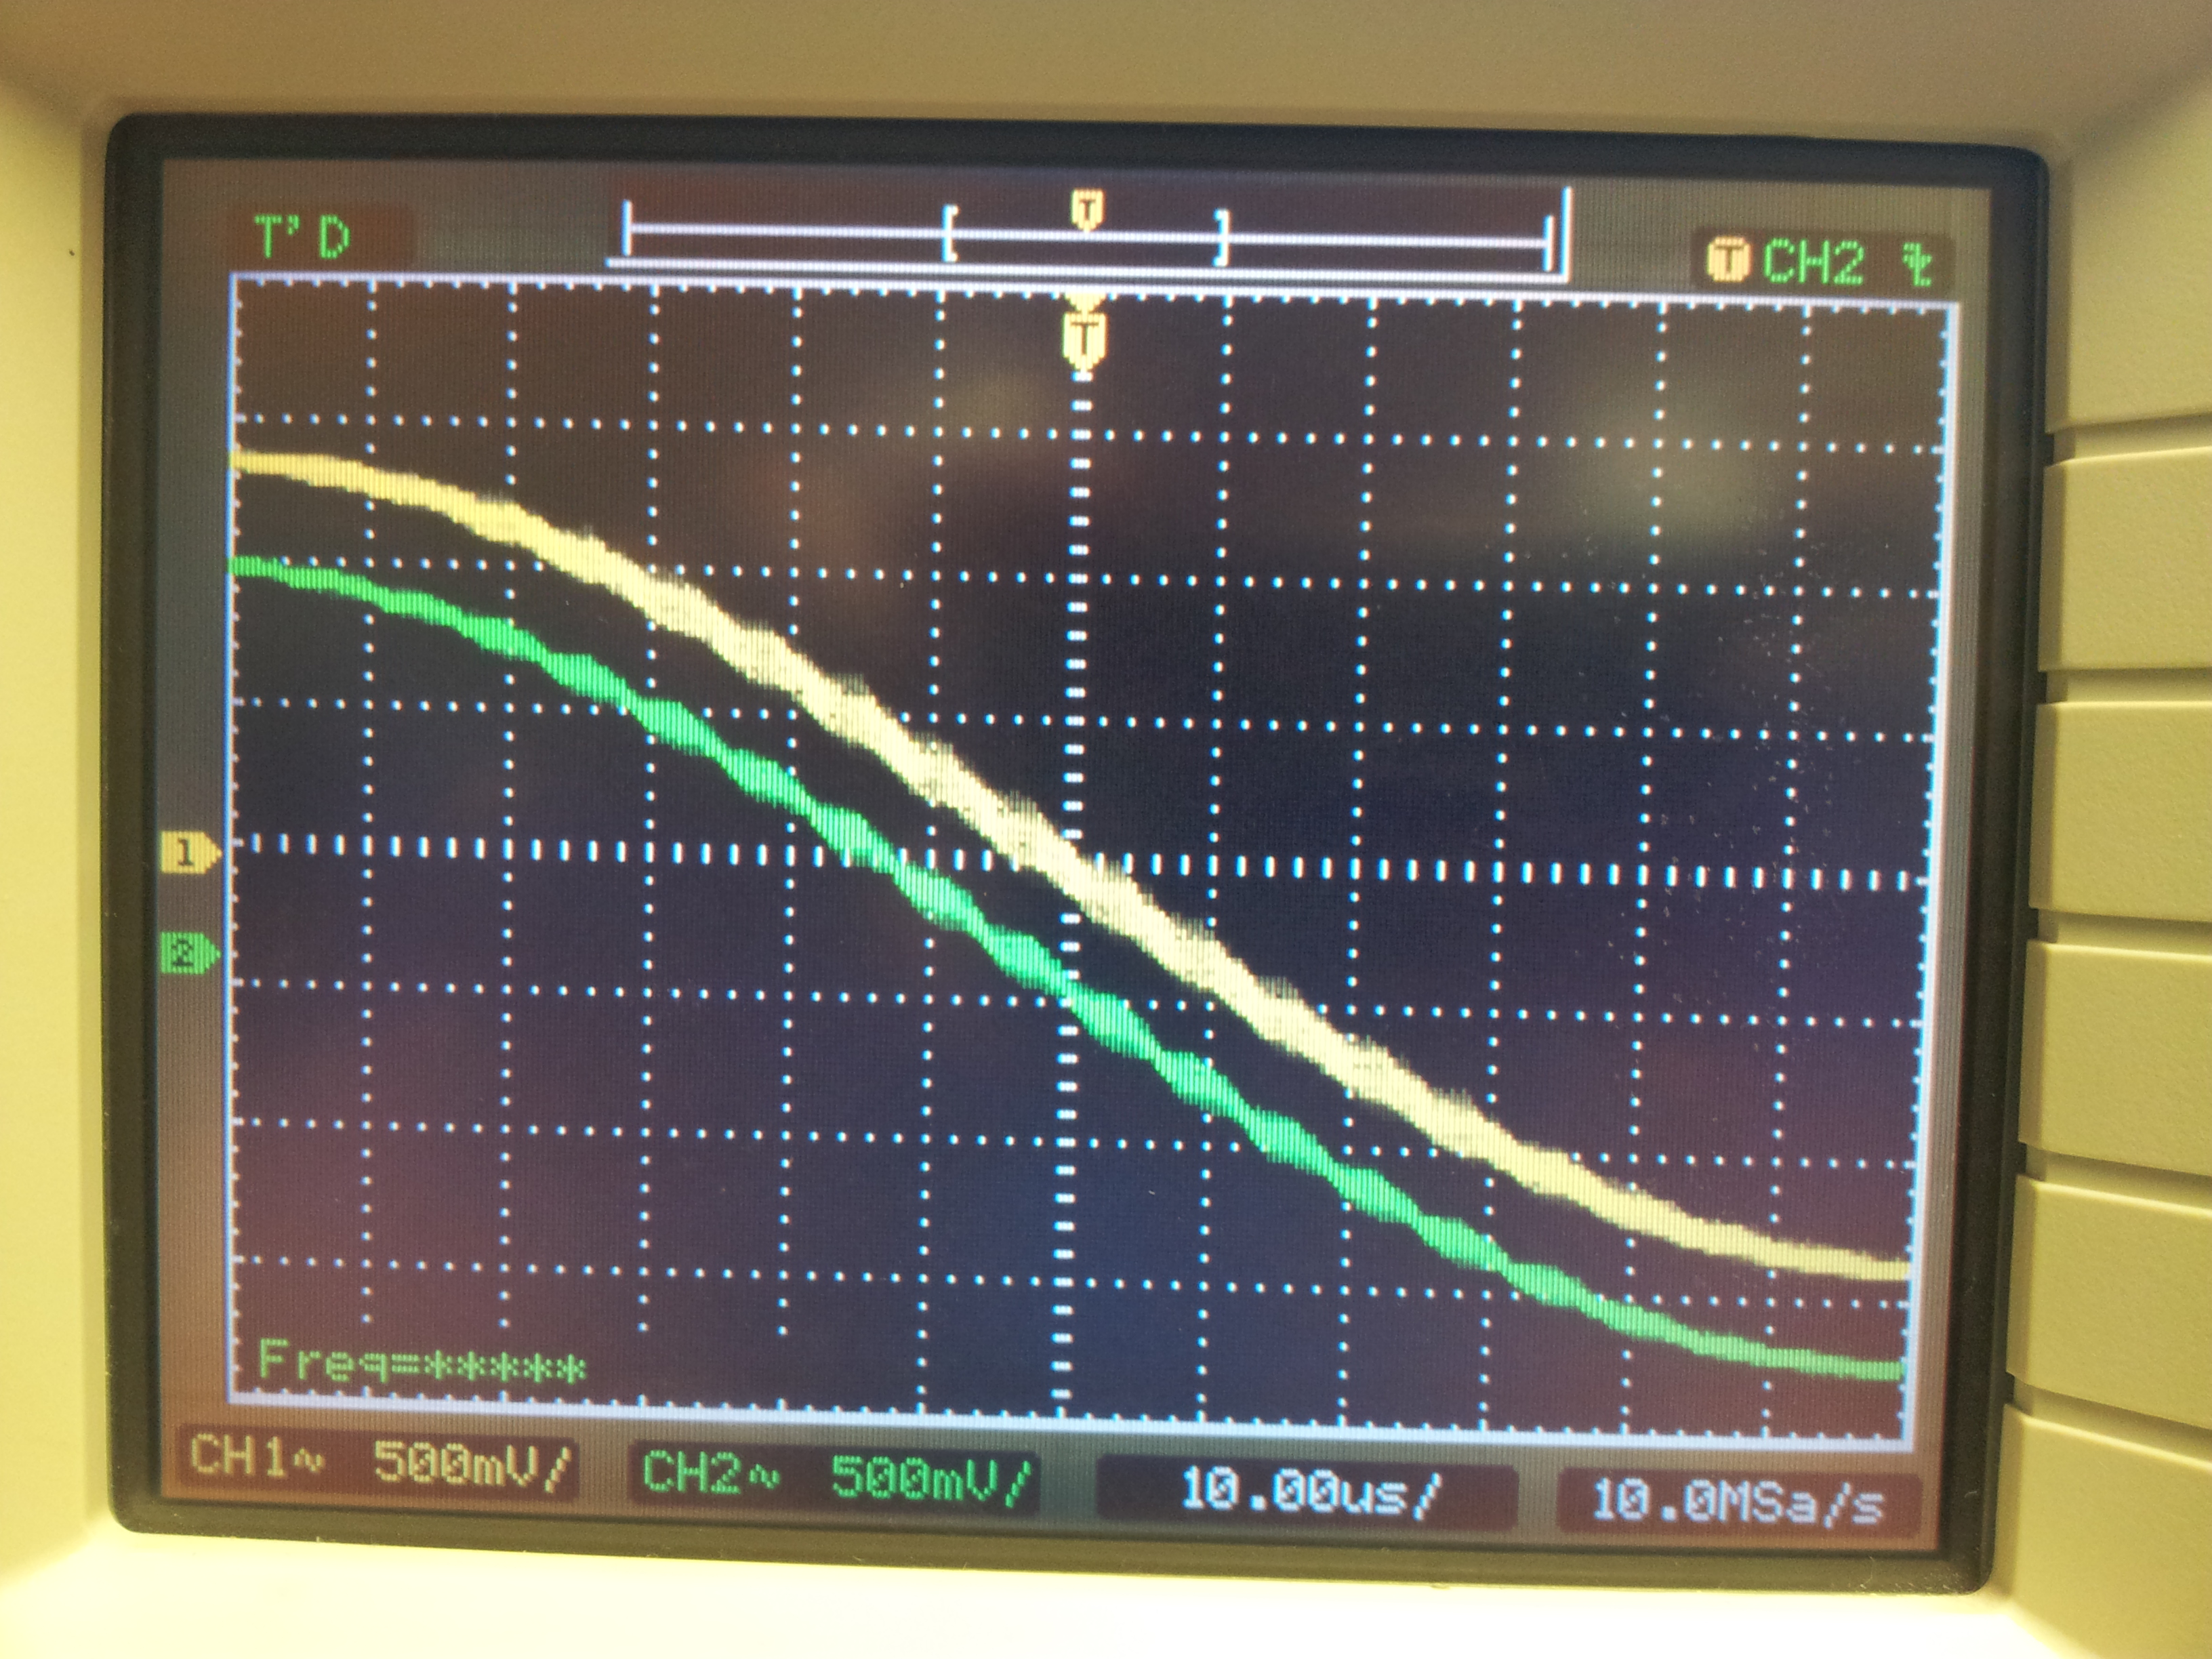
\includegraphics[width=0.5\textwidth]{./P1_interp}~\\
	\caption{Sinal sinusoide com interpolação e sem interpolação.}
	\label{fig:interp}
\end{figure}
Nesta figura é possível observar os "degraus" mencionados anteriormente, tanto na onda interpolada como na onda não interpolada.
\vspace{2 mm}

\textbf{P1-8}

Não sendo possível estabelecer uma diferença entre os sinais com interpolação e sem interpolação foi necessário recorrer à observação dos espectros deles mesmos (Figuras \ref{fig:espect_s_interp} e \ref{fig:espect_c_interp}).

\begin{figure}[H]
	\centering
	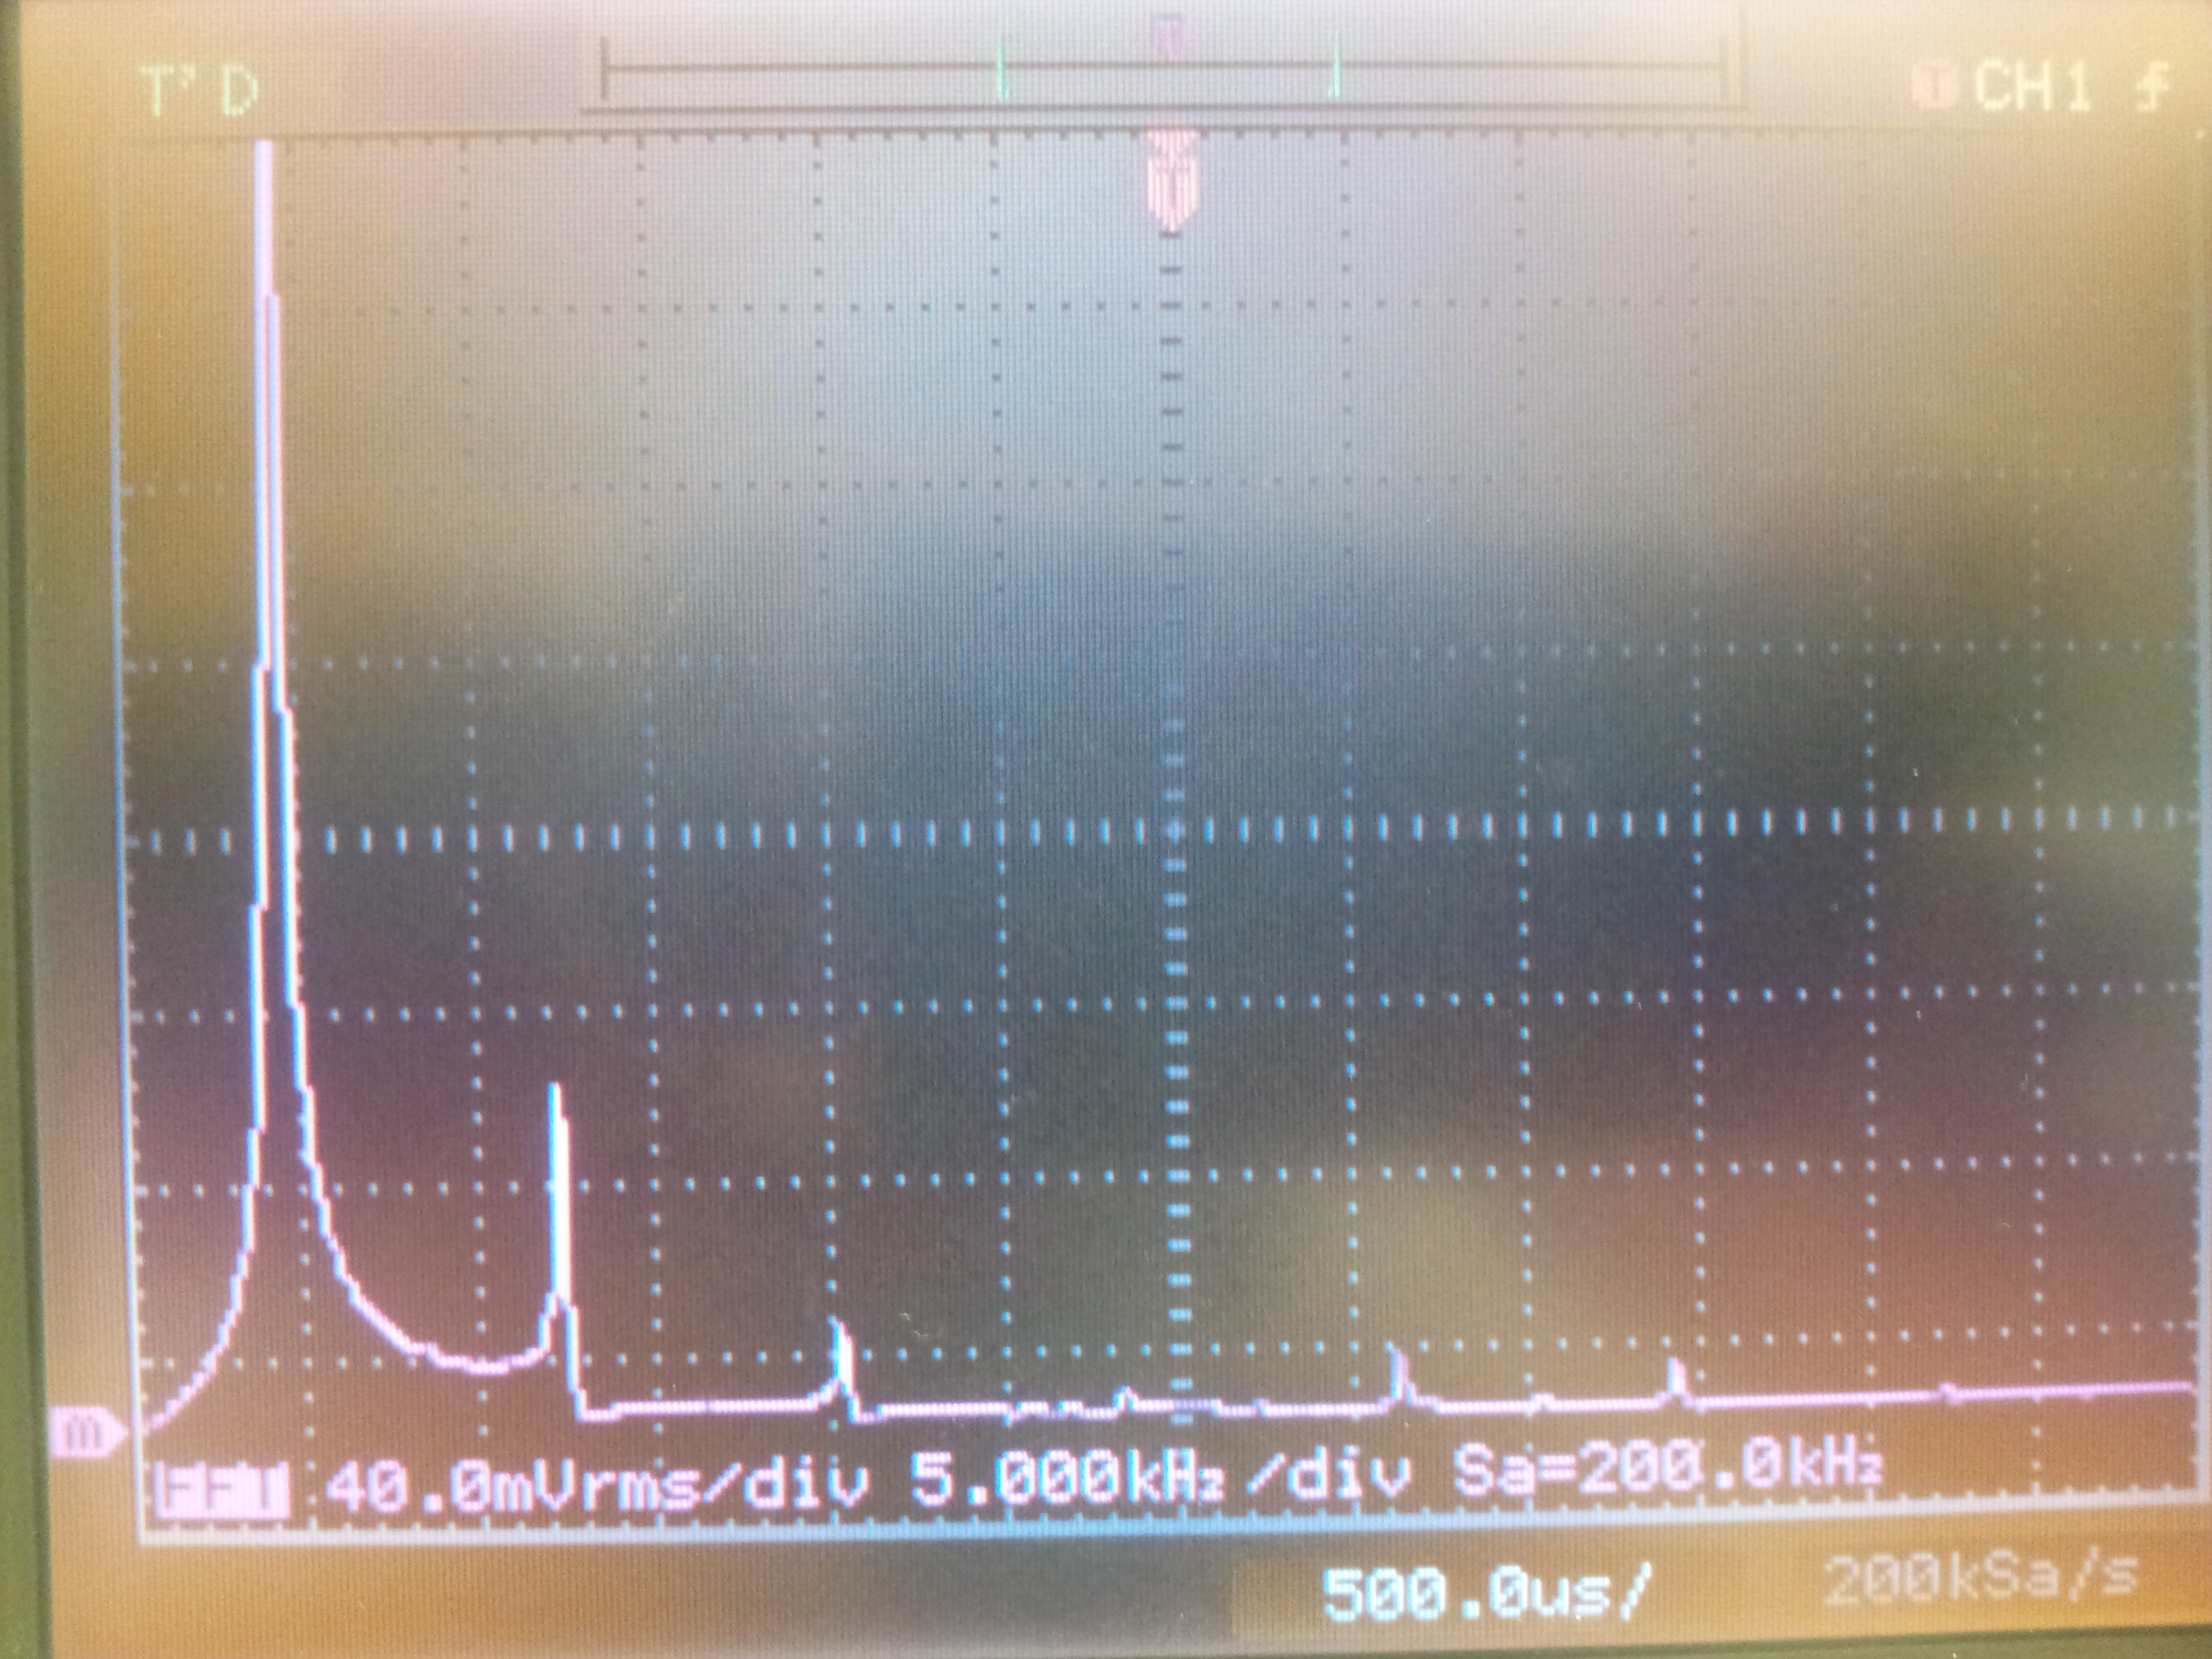
\includegraphics[width=0.5\textwidth]{./P1-8_espect_s_interp}~\\
	\caption{Espectro do sinal sinusoide sem interpolação.}
	\label{fig:espect_s_interp}
\end{figure}

\begin{figure}[H]
	\centering
	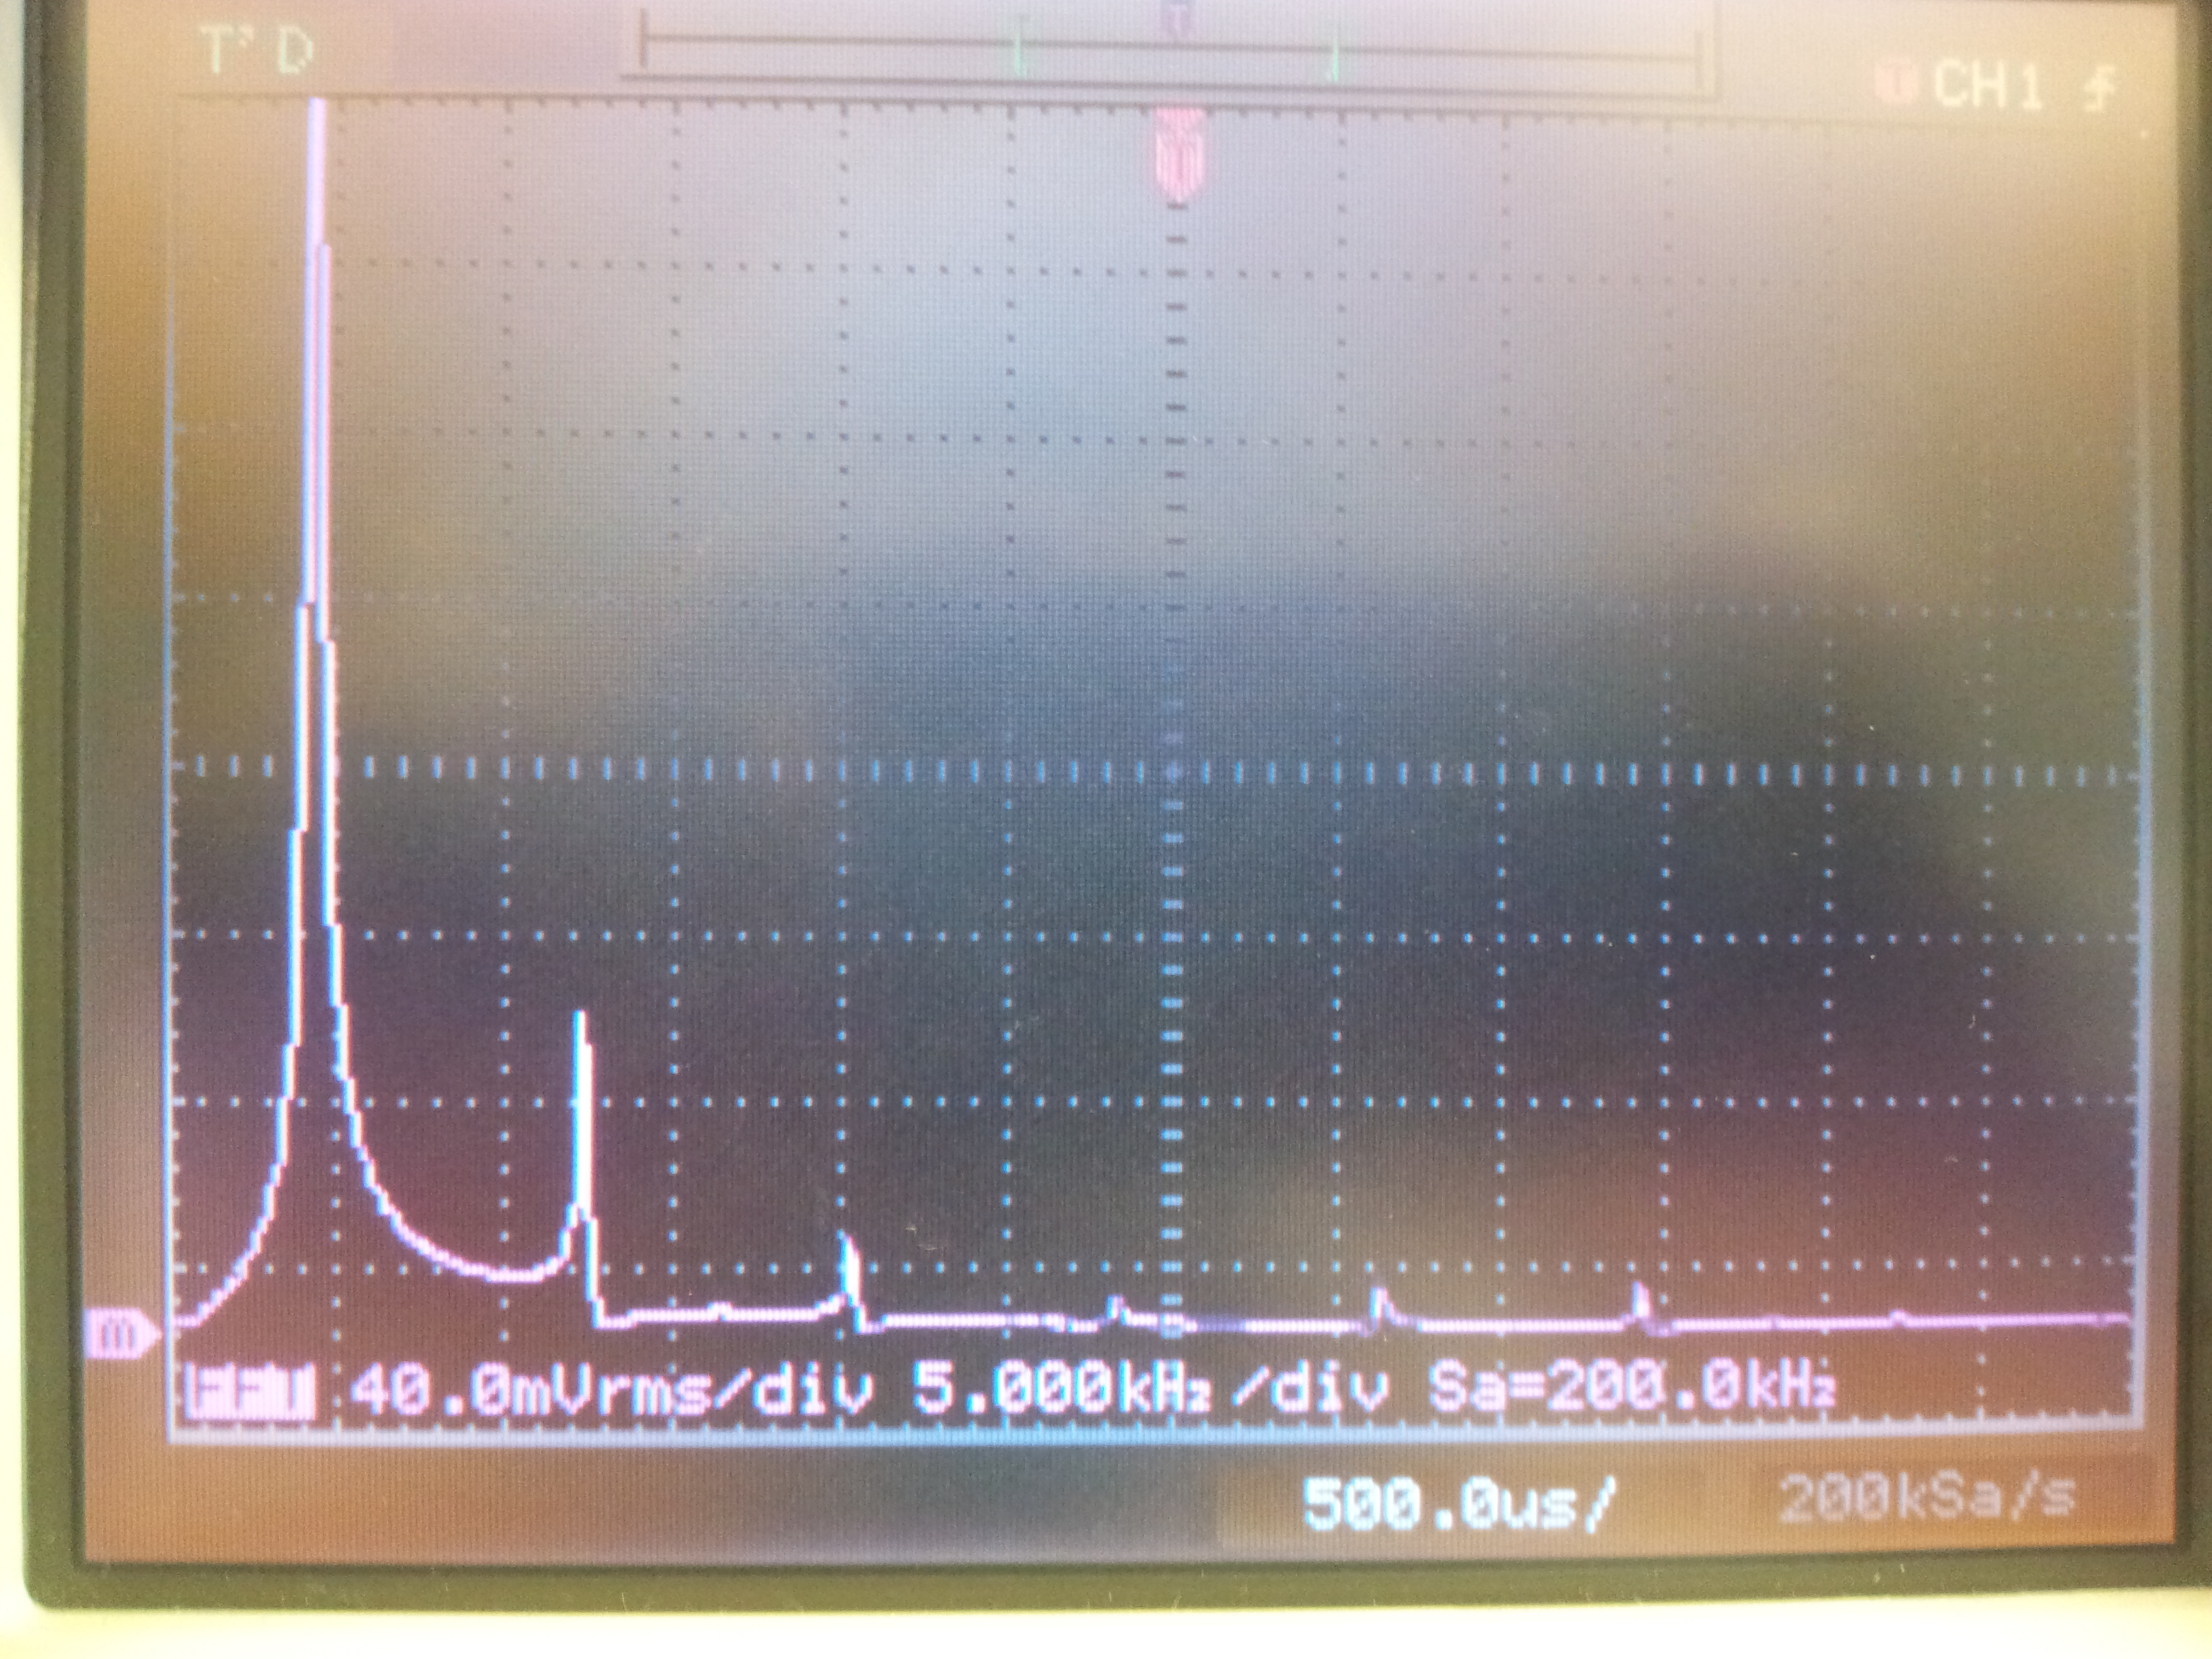
\includegraphics[width=0.5\textwidth]{./P1-8_espect_c_interp}~\\
	\caption{Espectro do sinal sinusoide com interpolação.}
	\label{fig:espect_c_interp}
\end{figure}

De novo não foi possível observar nas figuras diferenças visíveis entre os dois sinais, desta vez entre os seus espectros. Apresentam aparentemente a mesma amplitude para cada frequência entre eles mesmos.

A conclusão que se pode tirar com estas observações é que o método de interpolação, embora apresente uma melhor precisão dos valores, não apresenta uma melhoria nos resultados, sendo assim um método que apenas irá exaustar mais os recursos do processador sem obter qualquer tipo de retorno notável. Podemos então concluir que caso seja preciso usar um sinal digital de uma sinusoide podemos usar apenas o método que não usa interpolação.

É de referir que não se está a excluir a hipótese da interpolação melhorar o sinal. É afirmado que os pontos têm uma melhor precisão, mas as melhorias não são observáveis pelos métodos e equipamentos usados.

\subsubsection{P2. Transmissor BPSK}

%Introdução Teórica
O objectivo deste projeto é criar um transmissor BPSK com recurso a três elementos principais, uma fonte de bits, um codificador diferencial e mapeador, e um modulador.
Neste projeto foi utilizada uma frequência de amostragem $f_s=16$ kHz e uma frequência portadora $f_0=4$ kHz.

\vspace{2 mm}

\textbf{P2-1}

Para ter uma fonte de bits no transmissor usa-se um "bit-rate clock" cuja função vai ser criar uma sequência de bits $ b_n $ com $f_b=1$ kbps. Isto significa que, considerando $f_s$, a cada 16 ciclos é gerado um novo bit, alternado em relação ao anterior. Assim, implementou-se um contador que é incrementado em cada ciclo  e que tem uma condição para verificar quando chegar ao valor 16. Ao entrar nessa condição é implementada a lógica para cálculo do novo bit da sequência e o contador é reiniciado.

Para calcular o novo bit, basta negar o bit anteriormente obtido para obter uma sequência de bits alternada, tendo sido concretizado através de uma simples XOR:
\begin{equation}
b_n=b_{n-1} \oplus 1
\end{equation}
Com esta operação, o bit resultante será sempre alternado em relação ao anterior.
Assim, obtém-se uma onda quadrada, observada no osciloscópio, que varia entre "0" e "1" e representa $ b_n $  com uma frequência de $500$ Hz(ver figura com bn). Esta frequência ocorre devido a dividir-se  $f_b$ por dois pois cada meio ciclo da onda quadrada corresponde a um bit.  
\vspace{2 mm}

Após obter a fonte de bits passou-se ao segundo elemento do transmissor: o codificador diferencial e mapeador. Começando pelo codificador diferencial, este serve para evitar ambiguidades na fase de maneira a poder sempre recuperar uma sequência de bits num canal que tenha sofrido uma variação na fase.
A codificação de $b_n$ resulta também de uma operação lógica XOR, como se pode observar: 
\begin{equation}
c_n=c_{n-1} \oplus b_n \hspace{3 mm} ,c_0=0
\end{equation}
Como um bit novo só é calculado quando o contador chega ao valor $16$, o mesmo também só é codificado nessa condição, ou seja, a cada 16 ciclos é codificado um bit. 

Tal como em $ b_n $ também $ c_n $ é representado por uma onda quadrada que varia entre "0" e "1" só que com o dobro do período, devido a só ter dois resultados para os quatro casos possíveis da XOR que realiza a codificação(Figura \ref{bn_cn}).

\begin{figure}[H]
	\centering
	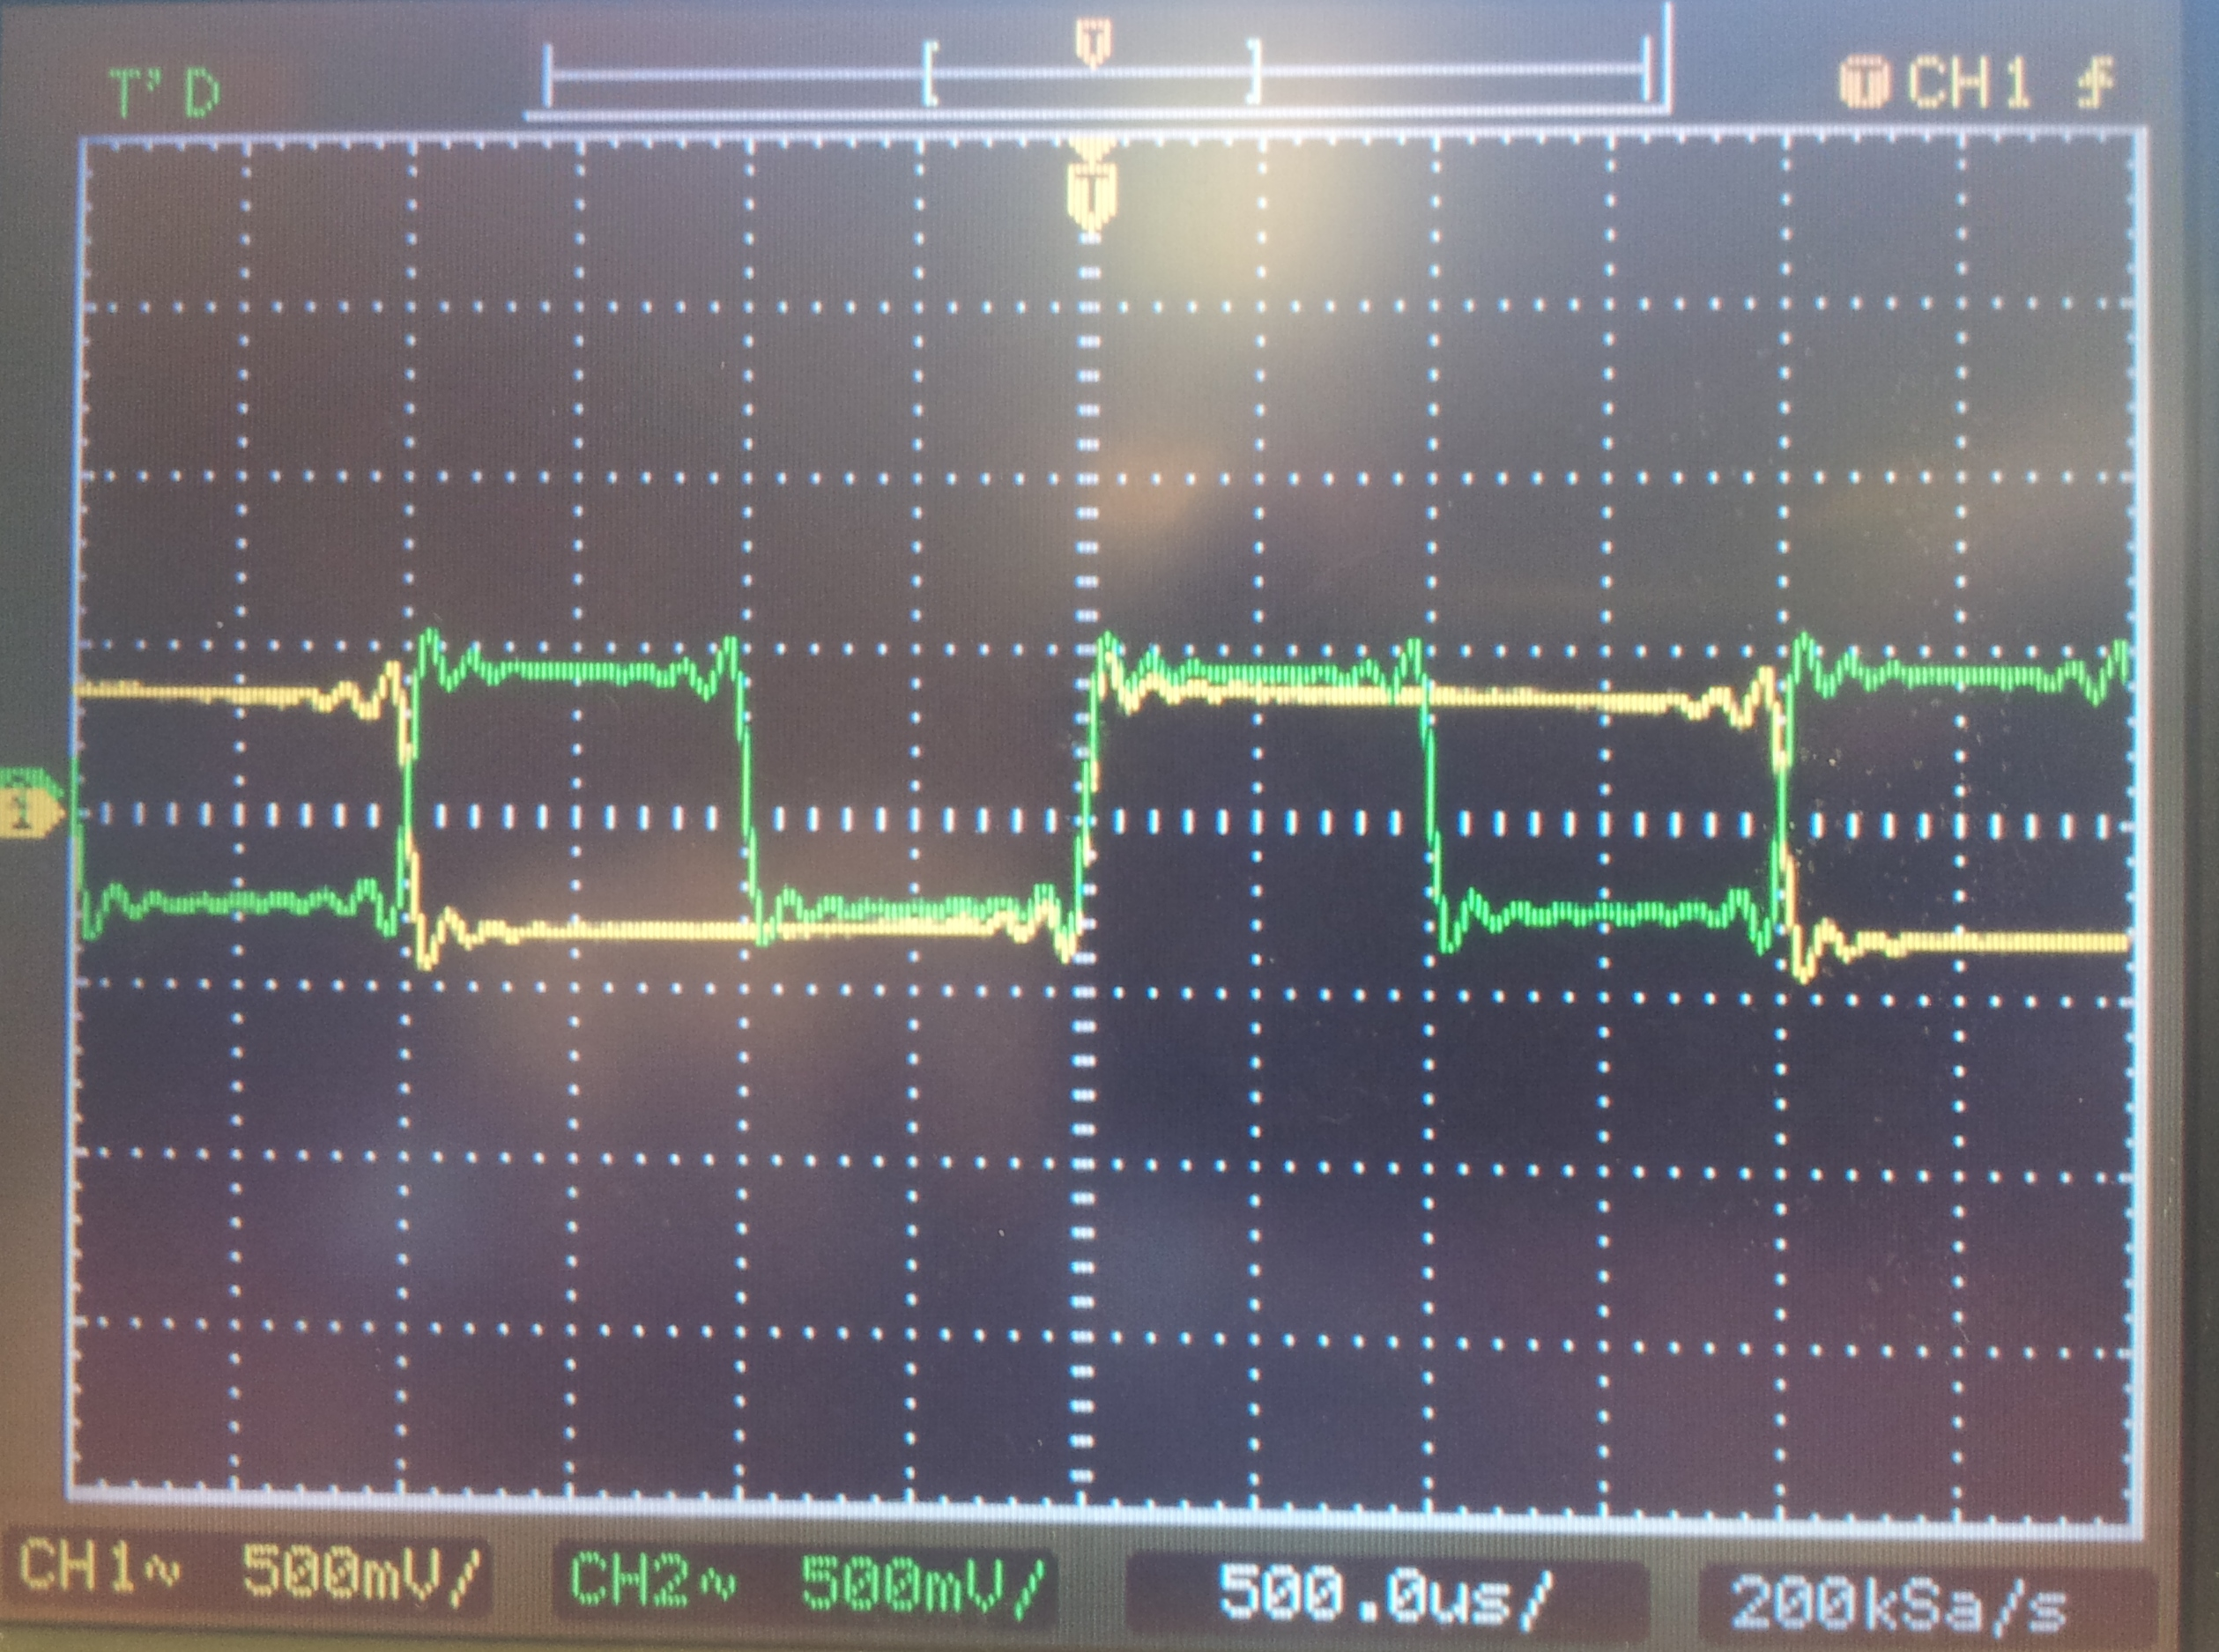
\includegraphics[width=0.5\textwidth]{./bn_cn}~\\
	\caption{$ b_n $(verde) e $ c_n $(amarelo)}
	\label{bn_cn}
\end{figure}

Depois de obter $ c_n $ passa-se ao mapeamento do mesmo. O mapeamento baseia-se em duas condições:
\begin{equation}
	c_n= '1' \rightarrow d_n =+1 \hspace{5 mm} c_n='0' \rightarrow d_n=-1
\end{equation}
Esta lógica podia ser facilmente implementada com recurso a duas condições "if", mas optou-se por evitar essa lógica para tornar o programa mais eficiente.
Assim recorreu-se a um \textit{shift} e a uma subtração. Atenção que esta não é a maneira mais eficiente pois a subtração faz com que o programa tenha de passar pela ALU.
Pode-se observar então o mapeamento efetuado através da seguinte expressão:
\begin{equation}
d_n=32767*((c_n << 1)-1)
\end{equation}
Antes de mais, o ganho que está a ser multiplicado é utilizado para converter o resultado em Q15, como já foi feito anteriormente. Considerando a expressão sem esse ganho, vê-se que para $ c_n=0 $, como o \textit{shift} não influencia o resultado, o mesmo só depende da subtração e é sempre o pretendido, $d_n=-1$. Se $c_n=1$, o \textit{shift} duplica  esse valor, e depois ao subtrair obtém-se $d_n=1$.

Tal como em $b_n$ e $c_n$ esta operação só é executada a cada 16 ciclos pois depende diretamente de $c_n$ e só se mapeia um novo bit depois de ele ser codificado. Concluído o mapeamento obtém-se mais uma vez uma onda quadrada mas desta vez varia entre "-1" e "1" (Figura \ref{cn_dn}).
\begin{figure}[H]
	\centering
	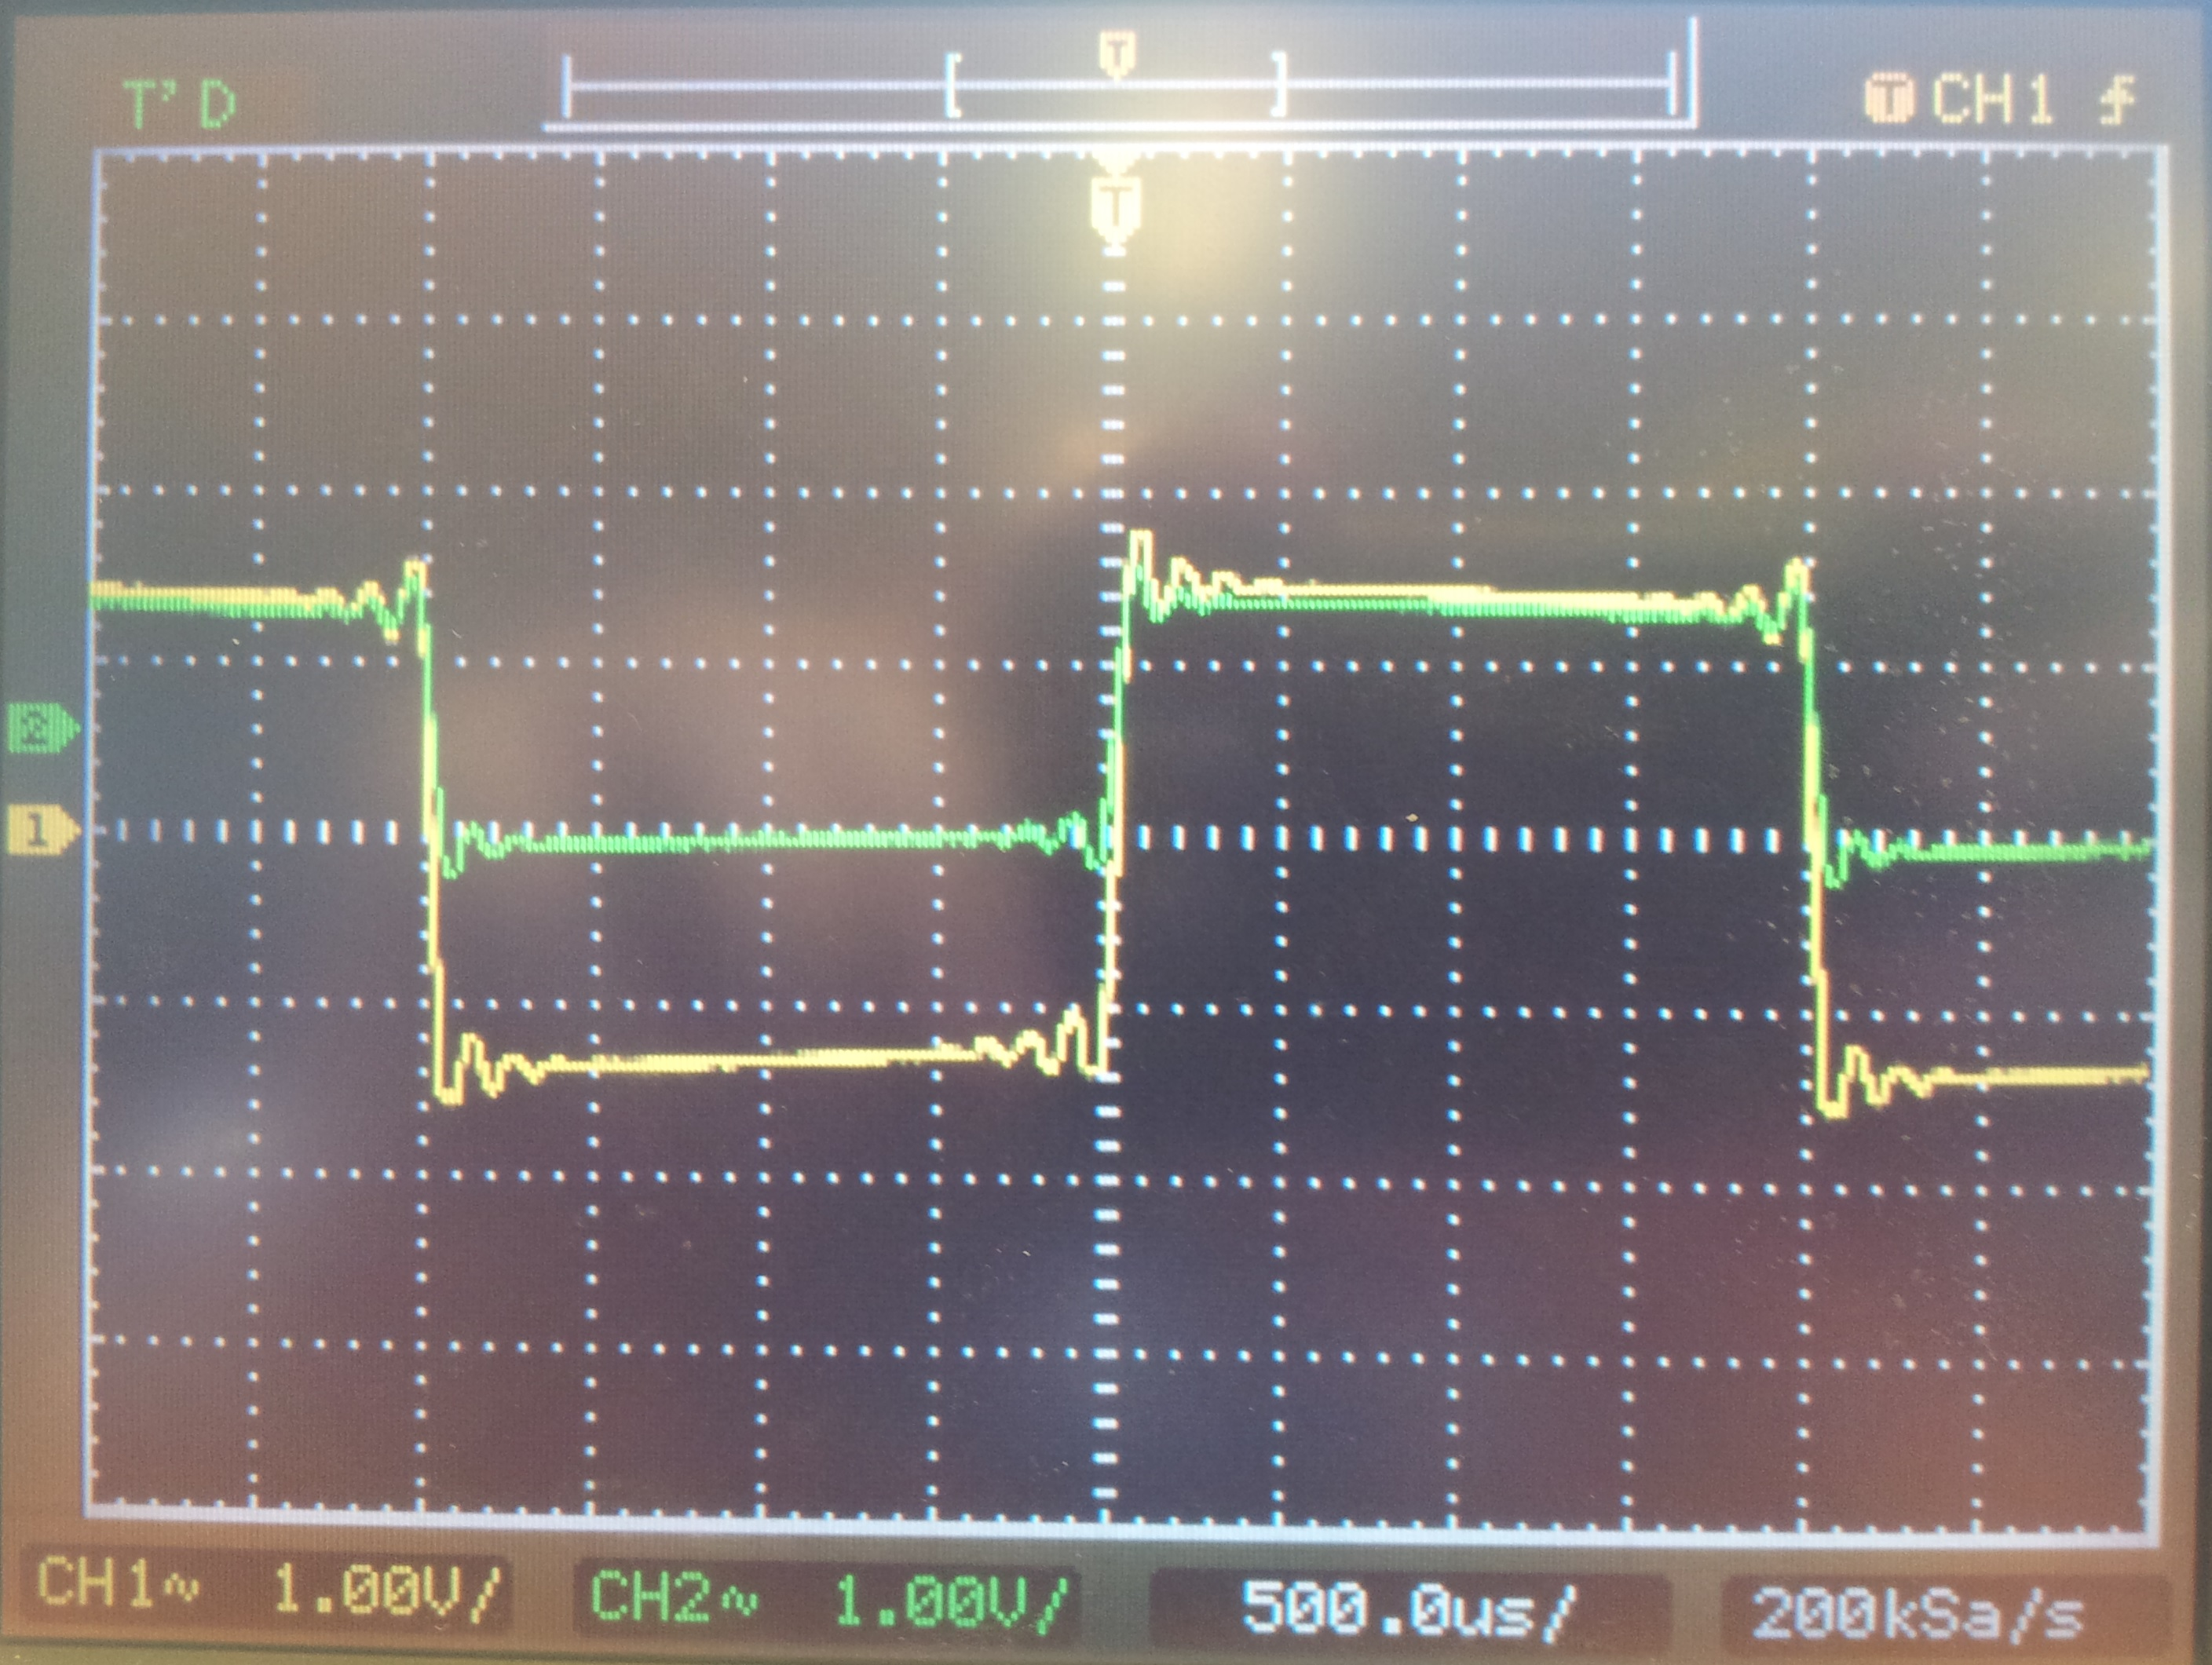
\includegraphics[width=0.5\textwidth]{./cn_dn}~\\
	\caption{$ c_n $(verde) e $ d_n $(amarelo)}
	\label{cn_dn}
\end{figure}
\textbf{P2-2}

Falta agora gerar a onda portadora a modular. Esta foi implementada de forma mais simples face ao projeto anterior uma vez que a frequência é estática (4 kHz) e este valor consiste numa fração inteira da frequência de amostragem ($16 kHz$).
Em primeiro lugar criou-se uma tabela com quatro valores dum período da sinusoide, sendo esta:
\begin{table}[H]
	\centering
	\caption{Amostras da onda portadora}
	\label{tab:amostras}
	\begin{tabular}[c]{|l||c|}
		\hline \textbf{contador} & \textbf{seno}\\ 
		\hline $ 0 $ & $ 0 $\\ 
		\hline $ 1 $ & $ 32767 $  \\ 
		\hline $ 2 $ & $ 0 $ \\ 
		\hline $ 3 $ & $ -32767 $ \\
		\hline
	\end{tabular}
\end{table}

Escolheram-se estes valores uma vez que o período de amostragem coincide com os instantes de máximo, mínimo e zero-crossing da portadora. Para gerar a portadora (Figura \ref{port_mod}) recorreu-se a um contador que, em cada interrupção (ocorrendo em cada instante de amostragem, como explicado no enunciado), aponta para cada entrada da tabela e põe a amostra numa variável que, após se incrementar o contador, irá ser multiplicada por $d_n$. Esta tabela não gera uma onda triangular pois das harmónicas destas, abaixo da frequência de amostragem ( $f_0$=4kHz e 3$f_0$=12kHz) apenas a primeira harmónica se encontra na banda de passagem do filtro de reconstrução do DAC, que terá frequência de corte Fs/2.

A onda modulada é então representada pela seguinte expressão:
\begin{equation}
	s_n= d_n \sin(2 \pi f_0T_sn) 
\end{equation}
Neste caso os valores do seno são os valores das amostras discutidas anteriormente.
\vspace{2 mm}

\textbf{P2-3}

Após implementar o modulador, tem-se o transmissor BPSK completo e para testá-lo, pôs-se nos dois canais do osciloscópio a onda portadora e a onda modulada (Figura \ref{port_mod}).

\begin{figure}[H]
	\centering
	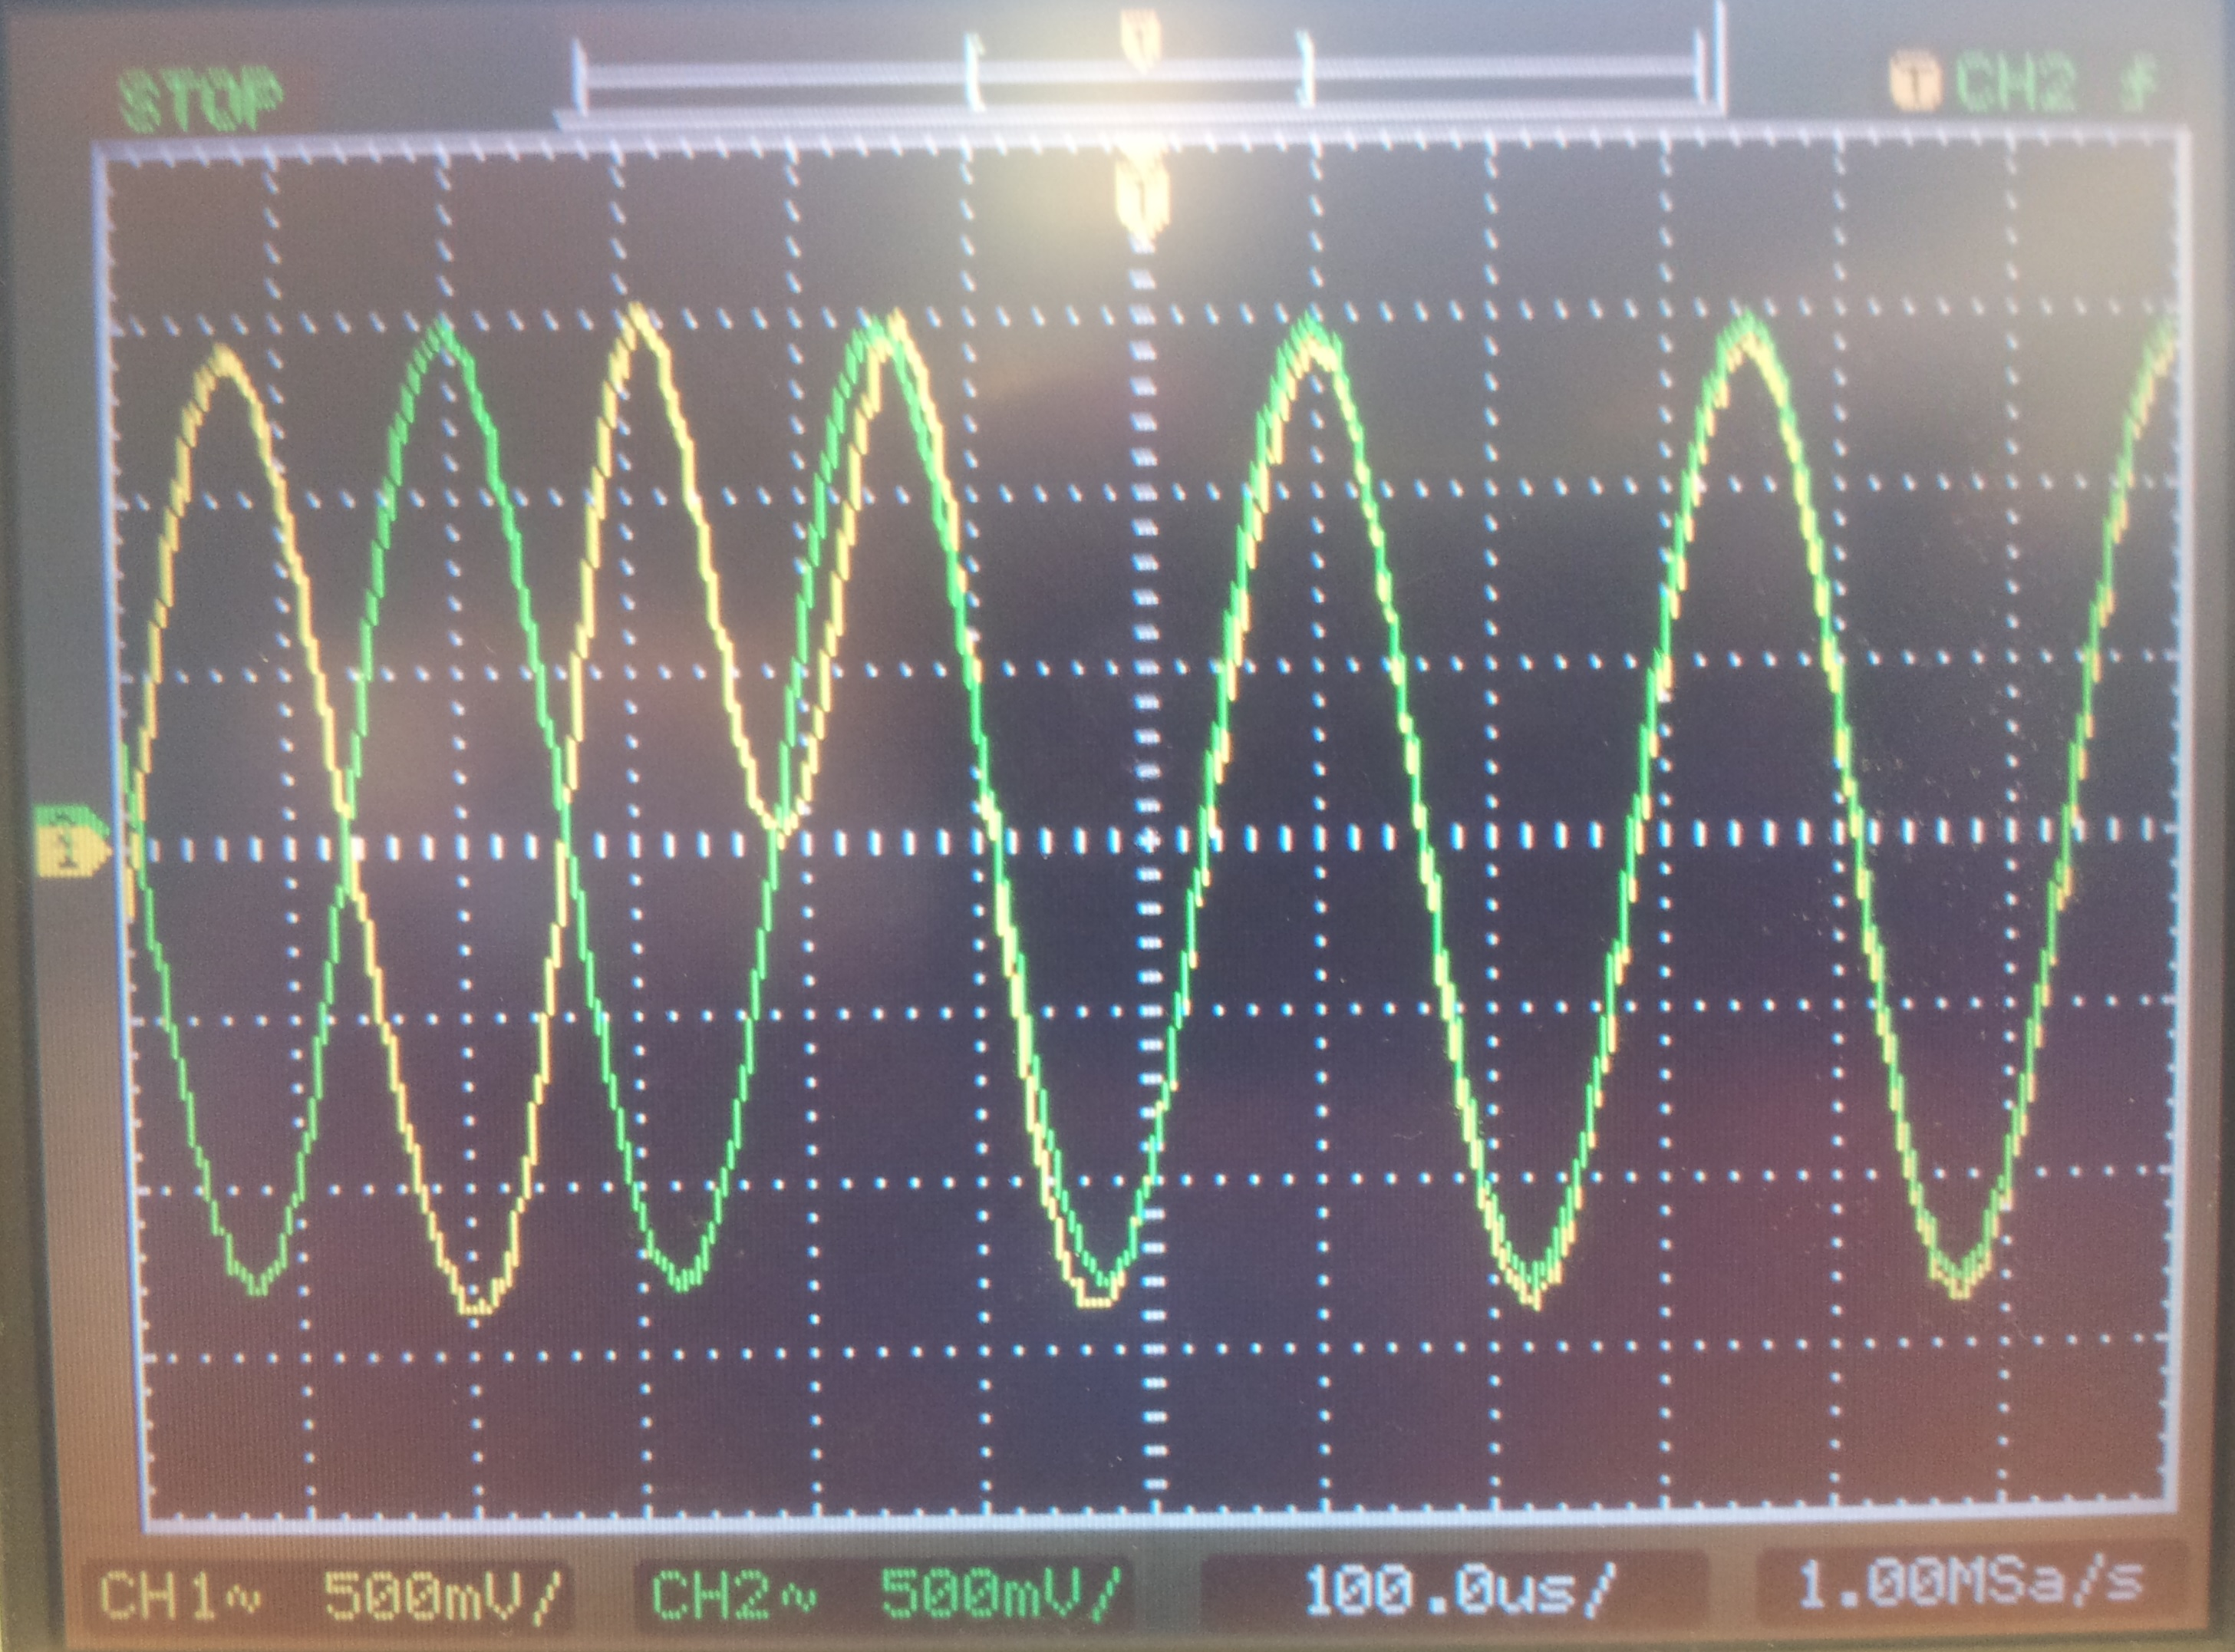
\includegraphics[width=0.5\textwidth]{./port_mod}~\\
	\caption{Onda portadora (verde) e onda modulada (amarelo)}
	\label{port_mod}
\end{figure}

Como se pode observar pela imagem e considerando a expressão (8), a onda portadora começa em oposição de fase com a onda modulada. Isto ocorre quando $d_n=-1$, o que significa que quando $d_n=1$ a onda modulada é igual à portadora. É possível observar quando $d_n$ muda de valor pois é exatamente quando a onda modulada inverte a sua direção (Figura \ref{dn_mod}). 

\begin{figure}[H]
	\centering
	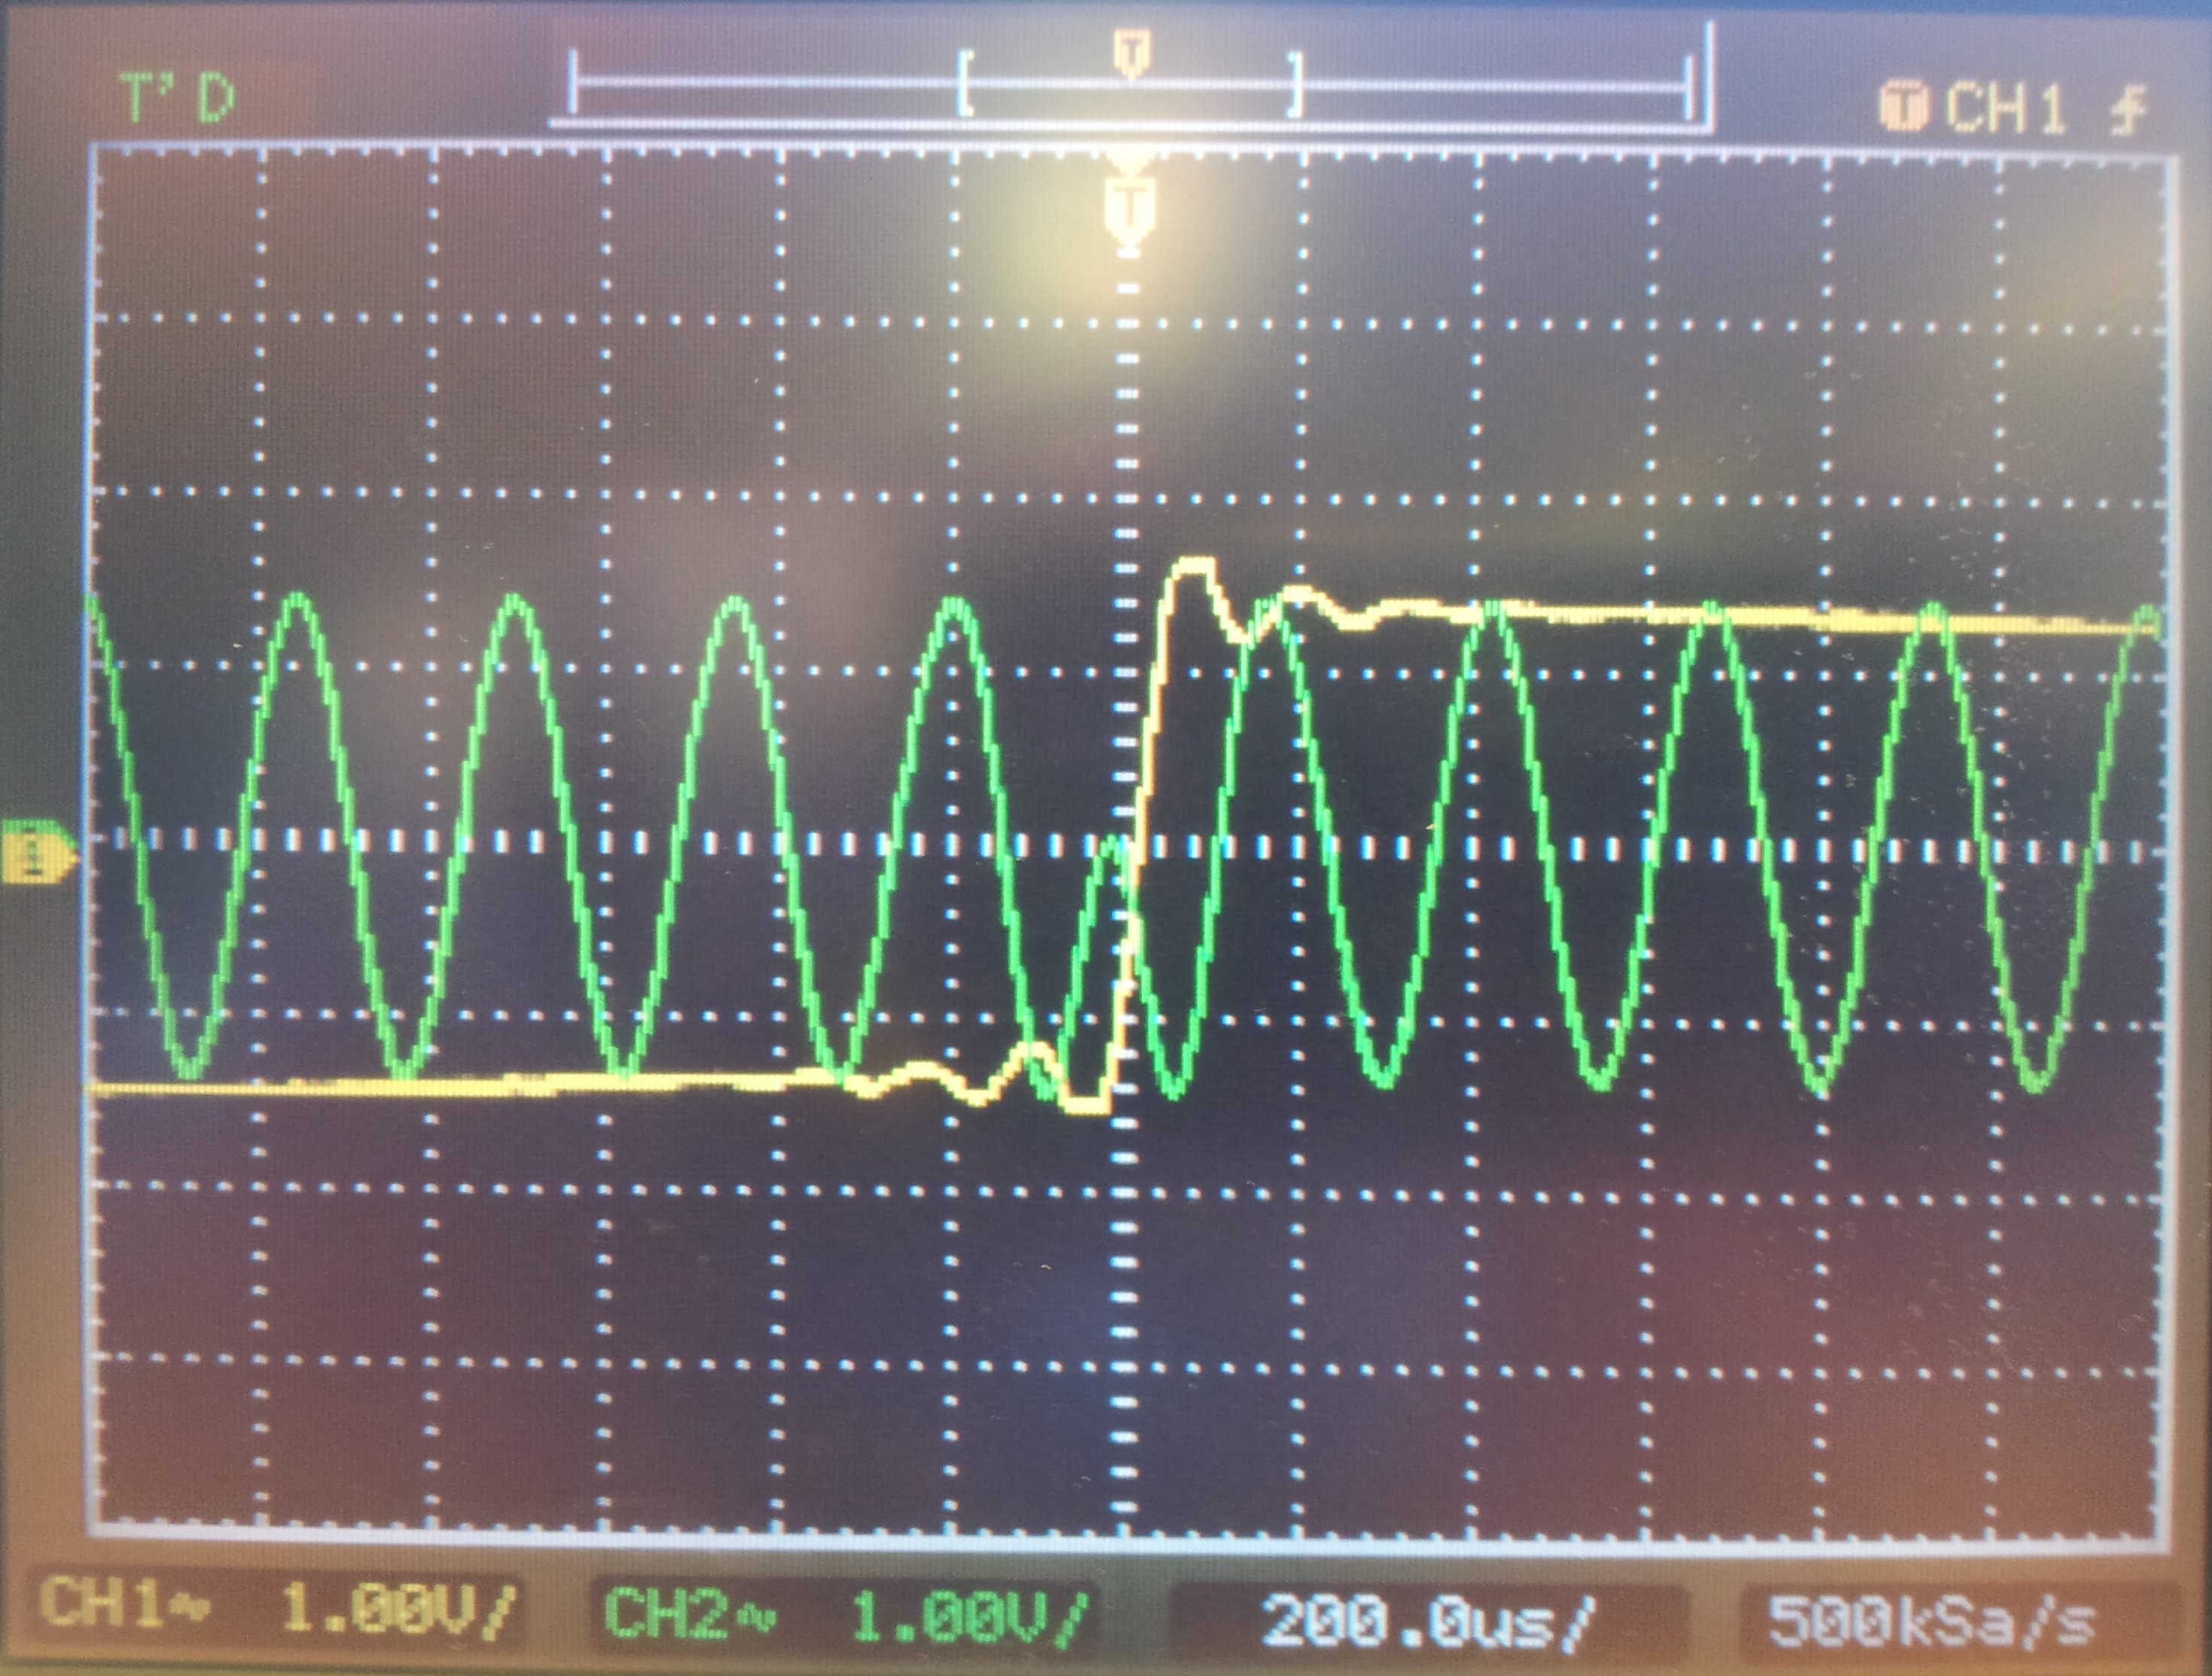
\includegraphics[width=0.5\textwidth]{./dn_mod}~\\
	\caption{Onda modulada (verde) e $d_n$ (amarelo)}
	\label{dn_mod}
\end{figure}

Este fenómeno acontece a cada 8 períodos do sinal modulado pois como já foi explicado anteriormente tem-se um bit-rate dividido por dois para corresponder um bit a meio-ciclo de uma onda quadrada, o que significa que se mapeia um novo bit a cada 8 períodos. 
\vspace{2 mm}

Para compreender melhor o sinal modulado, observou-se o espetro do mesmo (Figura \ref{espetro}).

\begin{figure}[H]
	\centering
	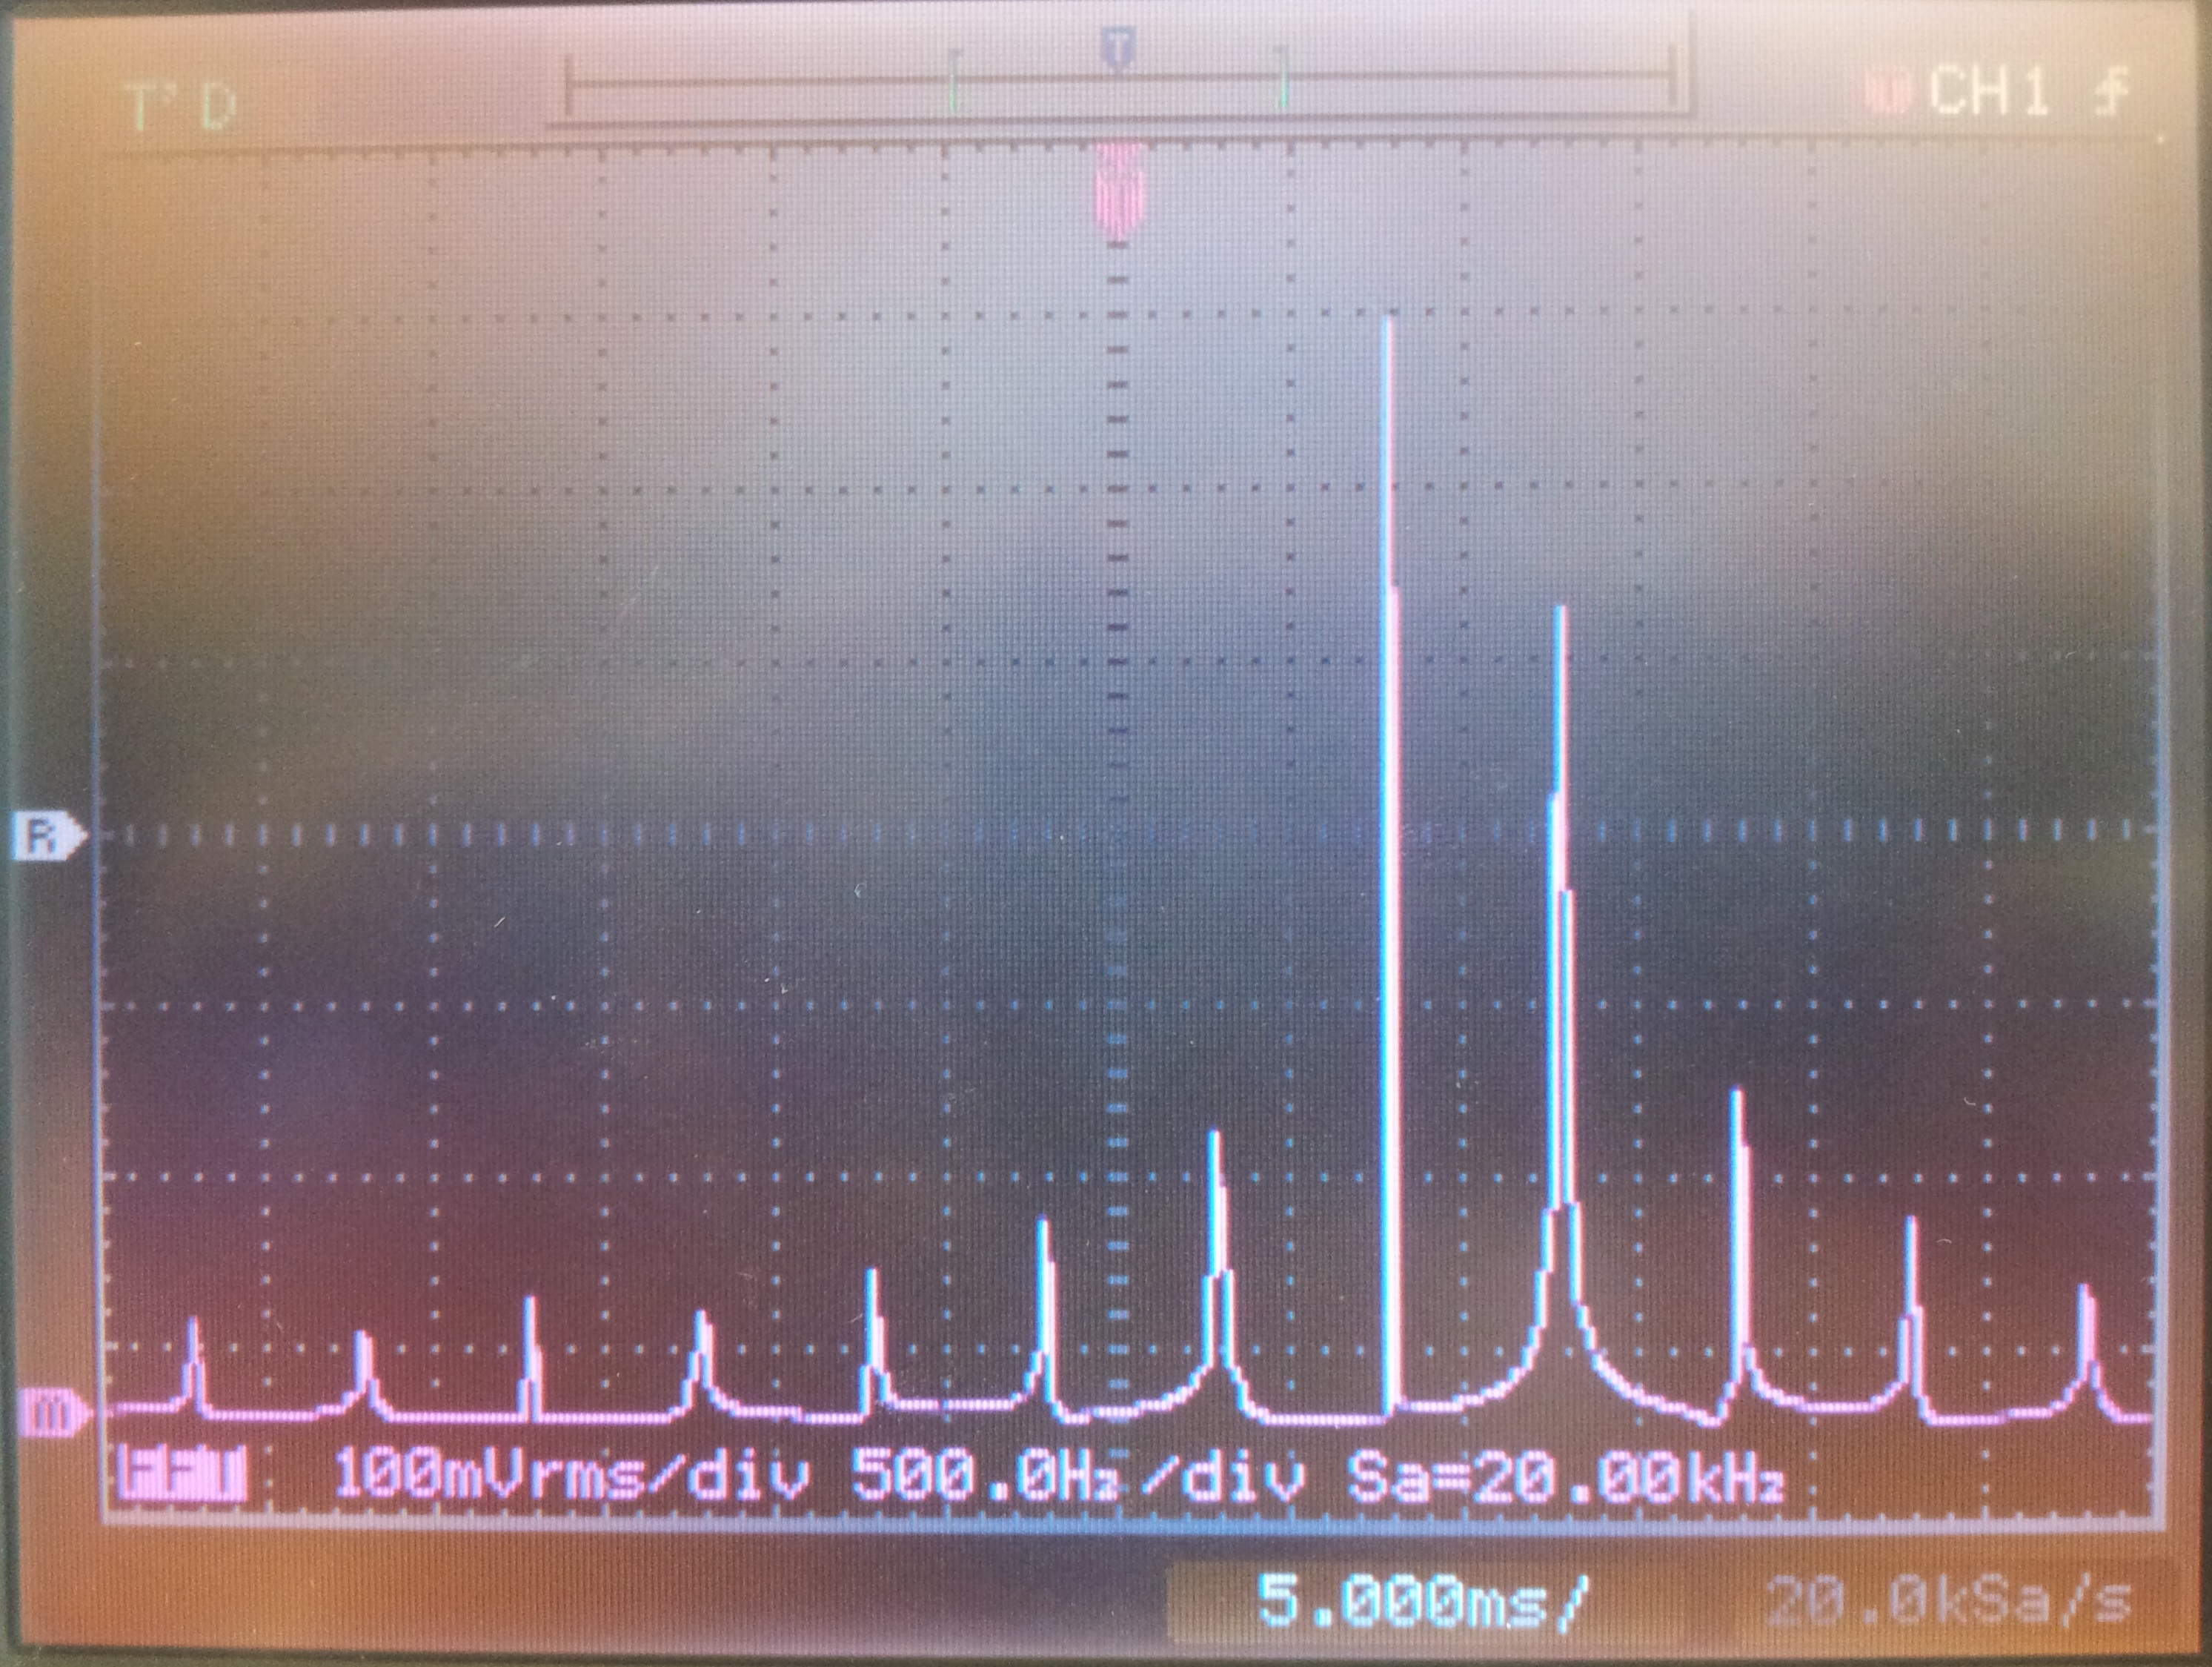
\includegraphics[width=0.5\textwidth]{./espetro}~\\
	\caption{Espetro da onda modulada}
	\label{espetro}
\end{figure}
A modulação da portadora com a onda quadrada, na frequência, faz a convolução das harmónicas ímpares (espectro quadrada) com um dirac a 4kHz (espectro da portadora).
Na Figura, o espectro da onda está mais centrado perto dos 4khz, como se esperava, onde se situam as harmónicas mais elevadas. Também se pode verificar que as harmónicas estão espaçadas por 500Hz pois o sinal $d_n$ consiste numa onda quadrada de frequência fundamental 250 Hz.
%melhorar

\section{Conclusão}
-Principais resultados e conclusões sobre eles, erros a corrigir (se houverem), o que melhorar

\section{Anexos}
-Codigo?

\end{document}